% ==========================================
% LatexRefinement Step Output: step4-2026-09-29-tuesday-week3-algebra-1-offset-final.tex
% Model: gemini-3.8-flash
% Temperature: 0.35
% TopP: 0.9
% TopK: 10
% MaxOutputTokens: 65535
% ThinkingBudget: 4096
% ThinkingLevel: HIGH
% Prompt Tokens: 72’032
% Candidates Tokens: 38’622 (inkl. Thinking Tokens)
% Cached Tokens: 0
% Processed on: 2026-10-04 13:15:25
% ==========================================

% Primary Language: English
% End of the video: 01:30:00

\lecturechapter[3]{Tuesday}{29 Sep}{29 September 2026}{Groups of Units, Fields of Fractions, and Polynomial Rings}
% Old chapter title: Rings, Groups of Units, and Fields of Fractions

\begin{overview}[Course Content Overview]
This lecture investigates the transition from commutative rings to fields and polynomials, focusing on the invertible elements of rings, the localization process that produces the minimal ambient field of an integral domain, and the algebraic construction of polynomial rings:
\begin{itemize}
    \item \textbf{The Group of Units $\operatorname{Unit}(R)$:} Structure of multiplicatively invertible elements, characterization of units in $\mathbb{Z}$ and the Gaussian integers $\mathbb{Z}[i]$ via the norm, and the group of units of residue class rings $(\mathbb{Z}/m\mathbb{Z})^*$.
    \item \textbf{Euler's Totient Function $\phi(m)$:} Definition as the order of $(\mathbb{Z}/m\mathbb{Z})^*$, with explicit computations for prime powers $\phi(p) = p-1$ and $\phi(p^2) = p(p-1)$.
    \item \textbf{Universal Property of $\mathbb{Q}$:} Rigorous formulation of $\mathbb{Q}$ as the smallest field containing $\mathbb{Z}$, and the unique extension of ring embeddings into fields.
    \item \textbf{Construction of the Field of Fractions $\operatorname{Frac}(R)$:} Generalization to arbitrary integral domains via equivalence classes of formal pairs $(x, y) \in R \times (R \setminus \{0\})$, verification of well-defined operations, and canonical embedding $i \colon R \hookrightarrow \operatorname{Frac}(R)$.
    \item \textbf{Concrete Quotient Fields:} Field of fractions of $\mathbb{Z}$, the Gaussian rationals $\mathbb{Q}(i) = \operatorname{Frac}(\mathbb{Z}[i])$, subrings of $\mathbb{Q}$ such as $\mathbb{Z}[\frac{1}{3}]$, and self-isomorphism for existing fields $\operatorname{Frac}(K) \cong K$.
    \item \textbf{Polynomial Rings $R[x]$:} Intuitive formulation via formal linear combinations, rigorous foundation using almost-zero sequences in $R^{\mathbb{N}_0}$, componentwise addition, and Cauchy product (convolution) multiplication.
\end{itemize}
\end{overview}

% --- TEIL 1 ---

\section{Review: Rings and the Group of Units}

\begin{speech}[00:00:00 - 00:00:32]
Okay, so we start. 

About the quiz: as I said, I'm very much pro-guessing in mathematics; you're never penalized for getting the wrong answer. Lika said that there was some implementation problem and some people were penalized for getting the right answer, and she's going to fix that, so. 

If you think the quiz was too easy, or too hard, or too medium, tell us. As I said, I've never gone through this quiz thing before. Okay, so then...
\end{speech}

\subsection{The Group of Units of a Ring}

\begin{speech}[00:00:32 - 00:01:51]
Last week we discussed rings, and associated to a ring there's an additive group. This is easy, because it's part of the definition, but there's another group which was also discussed in the last lecture (Recall: \cref{prop:group-of-units}), which is the group of units. 

And I remind you of this group... \inlinemetanote{writes \qt{the group of unit} $\operatorname{Unit}_R = \{ x \mid \exists y, xy = 1 \}$} Various people use different notation for describing it, but here I just say $\operatorname{Unit} R$ so there's no question: it's the group of units of the ring $R$. It's those elements such that there exists somebody else where the product is $1$, so it's those elements with a multiplicative inverse. And this is a group --- we discussed this last week. 

So, this group here is $\operatorname{Unit} R$, and it has, well, the units by this definition, multiplication, and $1$. \inlinemetanote{writes $\operatorname{Unit}_R = (\text{Units}, \cdot, 1)$}

Whenever you see a ring, you immediately have these two groups. And this one is, you know, often the more complicated one to think about, because it's not part of the definition in some sense.
\end{speech}

\begin{content}[The Group of Units]
\recap{Units and the group of units were introduced in Week~2 as $U(R)$ (\cref{def:unit-ring}, \cref{prop:group-of-units}); the lecturer now writes $\operatorname{Unit}(R)$.}

Let $(R, +, \cdot, 0, 1)$ be a ring with unity. Associated with $R$ are two natural canonical groups:
\begin{enumerate}[label=\textbf{(\arabic*)}]
    \item \textbf{The Additive Group:} $(R, +, 0)$, which forms an abelian group by the ring axioms.
    \item \textbf{The Group of Units:} The set of multiplicatively invertible elements in $R$:
    \begin{equation}\label{eq:unit-group-def-w3}
    \operatorname{Unit}(R) := \{ x \in R \mid \exists y \in R \text{ such that } xy = 1 \}.
    \end{equation}
\end{enumerate}

Under ring multiplication, $(\operatorname{Unit}(R), \cdot, 1)$ forms a group with identity element $1$.

\begin{steps}[Multiplicative Group Structure]
The group of units is closed under multiplication: if $x, z \in \operatorname{Unit}(R)$ with inverses $x^{-1}, z^{-1} \in R$, then $(xz)(z^{-1}x^{-1}) = 1$, so $xz \in \operatorname{Unit}(R)$. Associativity is inherited from the ring, and the multiplicative identity $1$ is invertible since $1 \cdot 1 = 1$.
\end{steps}
\end{content}

\subsection{Units in the Integers and Gaussian Integers}

\begin{speech}[00:01:51 - 00:03:03]
We've seen this --- I just review, but you know this --- if you take $\mathbb{Z}$, the units are $\pm 1$. And I said this many times, but maybe since I didn't actually ever give a proof: in $\mathbb{Z}[i]$, the units are $\pm 1, \pm i$ (Recall: \cref{exer:units-gaussian-integers}). 

If you're taking complex analysis, you should be able to prove this, but let's actually write a proof. I don't think I ever wrote the proof for this. 

So, proof: this is a proof that these are the only invertible elements in this ring. Is it clear what I'm trying to prove? 

Proof: let $a + bi \in \mathbb{Z}[i]$ be a unit. When I write this, of course that means that $a$ and $b$ are integers, okay? That's what being in there means. 

All right, so then there exists somebody else, $c + di$, also here, such that $(a+bi)(c+di) = 1$. And this is multiplication of complex numbers.
\end{speech}

\begin{speech}[00:03:03 - 00:03:58]
The whole idea of the proof is understanding multiplication of complex numbers. And if you've taken a complex numbers class, or you've met complex numbers, however you know it: when you multiply two complex numbers, their angles add and their lengths multiply, right? 

So, we just take the norm --- the lengths --- take the norms. The norm here is $\sqrt{a^2 + b^2}$; that's the length of this one. I hope that's not controversial, that's Euclid or something. This one is $\sqrt{c^2 + d^2}$, and their norms multiply, so this has to be just $1$. 

Okay? So, this is pretty restrictive: $a, b, c$, and $d$ are all integers.
\end{speech}

\begin{hidden}
% timestamp: 00:03:58
% topic: Determining units in the Gaussian integers Z[i] via norm multiplication
% board_state: eq:unit-group-def, units of Z, units of Z[i], norm equation
% next_goal: Deduce the 4 units (+-1, +-i) from the Diophantine equation a^2 + b^2 = 1 and draw the diagram
% open_loops: none
\end{hidden}

\begin{speech}[00:03:58 - 00:05:13]
So, we can square that equation: $(a^2+b^2)(c^2+d^2) = 1^2$, which is $1$. Now you have an equation where you have integers all multiplying to $1$, and you know the only way this can happen is if this integer itself is $\pm 1$, because you can't factor $1$ in the integers without having just $1 \cdot 1$ or $(-1) \cdot (-1)$. Is that clear? 

How could this be $1$? Well, $a^2$ for an integer is either $0$, or $1$, or something bigger. So, the only way this could be $\pm 1$ is if $a$ is equal to $0$ or $\pm 1$, and $b$ is equal to $0$ or $\pm 1$ --- those are the only cases. If these are both positive integers, it's going to be bigger than $1$. So, you only have to check these cases. Is that clear? 

And if you look at these cases, well, these are the answers. Okay? That's a complete proof; that's as complete a proof as you get in this class. I think this proof was $100$ percent complete. 

That's a nice fact, and if you draw them, they look like this \inlinemetanote{draws a sketch of the complex plane with four points on the axes}. Those are the four units in the Gaussian integers.
\end{speech}

\begin{content}[Classification of Units in the Gaussian Integers]
\recap{The units of $\mathbb{Z}$ were determined in Week~2 (\cref{ex:units-of-integers}), and those of $\mathbb{Z}[i]$ were stated in Week~1 and set as an exercise (\cref{exer:units-gaussian-integers}). The proof below settles that exercise.}

\begin{example}[Units of the Integers]\label[example]{ex:units-integers-w3}
For the ring of integers $\mathbb{Z}$:
\[
\operatorname{Unit}(\mathbb{Z}) = \mathbb{Z}^* = \{1, -1\}.
\]
\end{example}

\begin{proposition}[Units of the Gaussian Integers]\label[proposition]{prop:units-gaussian-integers}
The group of units of the Gaussian integers $\mathbb{Z}[i] = \{ a + bi \mid a, b \in \mathbb{Z} \}$ is:
\[
\operatorname{Unit}(\mathbb{Z}[i]) = \{1, -1, i, -i\}.
\]
\end{proposition}

\begin{proof}
Let $z = a + bi \in \mathbb{Z}[i]$ be a unit with $a, b \in \mathbb{Z}$. By definition, there exists $w = c + di \in \mathbb{Z}[i]$ ($c, d \in \mathbb{Z}$) such that:
\begin{equation}\label{eq:gaussian-unit-prod}
(a + bi)(c + di) = 1.
\end{equation}
Taking the complex modulus (Euclidean length) on both sides of \eqref{eq:gaussian-unit-prod}:
\[
|a + bi| \cdot |c + di| = |1| = 1 \implies \sqrt{a^2 + b^2} \cdot \sqrt{c^2 + d^2} = 1.
\]
Squaring this relation yields an equation in non-negative integers:
\begin{equation}\label{eq:norm-mult-equation}
(a^2 + b^2)(c^2 + d^2) = 1.
\end{equation}
Since $a^2 + b^2 \in \mathbb{Z}_{\ge 0}$ and divides $1$, we must have:
\[
a^2 + b^2 = 1.
\]
Because $a, b \in \mathbb{Z}$, the only integer solutions to $a^2 + b^2 = 1$ are:
\begin{align*}
a = \pm 1, \quad b = 0 &\implies z = \pm 1, \\
a = 0, \quad b = \pm 1 &\implies z = \pm i.
\end{align*}
Conversely, $1 \cdot 1 = 1$, $(-1)(-1) = 1$, and $i(-i) = 1$, so all four elements are invertible. Thus:
\[
\operatorname{Unit}(\mathbb{Z}[i]) = \{1, -1, i, -i\}.
\]
\end{proof}

\begin{center}
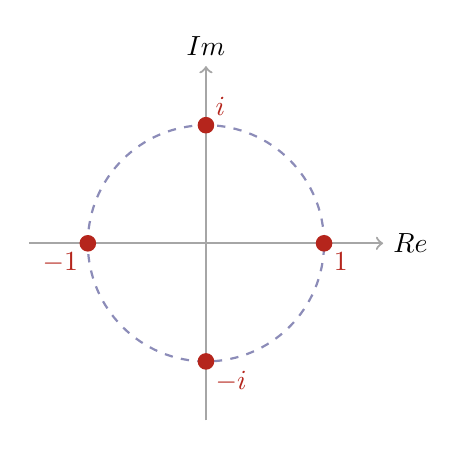
\begin{tikzpicture}[scale=1.5]
% \begin{hidden}
% - Canvas: scale=1.5, x in [-1.5, 1.5], y in [-1.5, 1.5]
% - Elements: coordinate axes, dashed unit circle, four unit points marked with labels
% - Coordinates: (1,0) for 1, (-1,0) for -1, (0,1) for i, (0,-1) for -i
% - Occlusion: axes in background, dashed circle in midground, dots and labels in foreground
% \end{hidden}
    % Axes
    \draw[->, thick, gray!70] (-1.5, 0) -- (1.5, 0) node[right, text=black] {$\operatorname{Re}$};
    \draw[->, thick, gray!70] (0, -1.5) -- (0, 1.5) node[above, text=black] {$\operatorname{Im}$};

    % Unit Circle (radius 1 coordinate unit)
    \draw[dashed, MidnightBlue!50, thick] (0,0) circle (1);

    % Four Units
    \fill[BrickRed] (1, 0) circle (2pt) node[below right, text=BrickRed, font=\bfseries] {$1$};
    \fill[BrickRed] (-1, 0) circle (2pt) node[below left, text=BrickRed, font=\bfseries] {$-1$};
    \fill[BrickRed] (0, 1) circle (2pt) node[above right, text=BrickRed, font=\bfseries] {$i$};
    \fill[BrickRed] (0, -1) circle (2pt) node[below right, text=BrickRed, font=\bfseries] {$-i$};
\end{tikzpicture}
\end{center}

\begin{steps}[Algebraic Meaning of the Norm]
The field norm $N(a+bi) = a^2 + b^2$ is multiplicative: $N(zw) = N(z)N(w)$. Since $N(z) \in \mathbb{Z}_{\ge 0}$ for any Gaussian integer, the norm of any invertible element must divide $N(1) = 1$, forcing $N(z) = 1$. The only lattice points on the circle of radius $1$ are the four points shown above.
\end{steps}
\end{content}

\subsection{Units in Residue Class Rings}

\begin{speech}[00:05:14 - 00:07:21]
We did a much more interesting example last time, which was also with proof, but since various people asked me about it afterwards, I want to do just another example. And that was this ring: $\mathbb{Z}/m\mathbb{Z}$. 

That's a nice ring, and so it has a group of units, $\operatorname{Unit}(\mathbb{Z}/m\mathbb{Z})$. This was a result I proved last time (Recall: \cref{thm:units-z-mod-m}): the units are equal to those classes such that this (i.e., $\gcd(x, m)$) is equal to $1$. And as I said, it's standard here to say $m \ge 2$, so we're not dealing with the zero ring, okay? 

So, that's the units, and these are the residue classes which are relatively prime. I did an example last time (Recall: $\mathbb{Z}/7\mathbb{Z}$, \cref{ex:units-z7z}). This is a very interesting thing to study; it's just not a trivial thing, in the sense that one might say that if I take the additive structure here, this is very simple to think about. It's just adding up integers mod $m$. In some sense, most people learn about this in one name or the other in school. 

But the units are more complicated, more interesting. And so I wanted to do another... there were various people who asked me some questions. So, let's try this: $\mathbb{Z}/10\mathbb{Z}$, just to say a little bit...

The standard notation for this is that: $(\mathbb{Z}/m\mathbb{Z})^*$. This is the usual notation for the units of $\mathbb{Z}/m\mathbb{Z}$. And also this notation is sometimes used in general: $R^*$ sometimes denotes the units, depending on the author. I've just been writing $\operatorname{Unit}$, so there's no question about what I mean, but in this case it's so common to use the star here that I'll also use the star. Is that clear?
\end{speech}

\begin{speech}[00:07:21 - 00:08:37]
How to think about this? Well, I'll just do an example, because as I said, there were various questions. How to think about this? This is all the residue classes that are relatively prime. So, you can just write them all first and cross them out: $0, 1, 2, 3, 4, 5$... maybe I should have picked something less than $10$... 

These are all the residue classes, and then we have to cancel all the ones that are not relatively prime. So, which ones? Is $0$ relatively prime? No, so we cross that out. $1$ is relatively prime; $1$ is always relatively prime. What about $2$? No. $3$? Yes, so we skip it. $4$? That has a $2$ in it, and $10$ has a $2$, so we cross that out. $5$? $10$ has a $5$ in it, so we cross that one out, cross that one out, and what's left? $4$, yeah. So, these are the four residue classes left. 

The group of units here consists of these residue classes, okay? And the claim is that this is a group under multiplication. That's what that claim is. So, for example, $3$ is in this group, so what is its inverse?
\end{speech}

\begin{student}[Student Answer]
$7$.
\end{student}

\begin{speech}[00:08:42 - 00:08:52]
Yeah, $7$, because $7 \times 3$ is $21$, and so on. So, anyway, you can play with this.
\end{speech}

\begin{hidden}
% timestamp: 00:08:45
% topic: Group of units in residue class rings Z/mZ and example Z/10Z
% board_state: eq:unit-group-def, def of (Z/mZ)^*, calculation of (Z/10Z)^* = {1, 3, 7, 9}
% next_goal: Introduce Euler's totient function phi(m) as the order of (Z/mZ)^*
% open_loops: none
\end{hidden}

\begin{content}[Units in \texorpdfstring{$\mathbb{Z}/m\mathbb{Z}$}{Z/mZ} and the Example \texorpdfstring{$\mathbb{Z}/10\mathbb{Z}$}{Z/10Z}]
\recap{This characterization was proved in Week~2 (\cref{thm:units-z-mod-m}); the lecturer restates it with the notation $(\mathbb{Z}/m\mathbb{Z})^*$.}

\begin{proposition}[Units in the Residue Class Ring]\label[proposition]{prop:units-mod-m-w3}
Let $m \in \mathbb{Z}_{\ge 2}$. The group of units of the residue class ring $\mathbb{Z}/m\mathbb{Z}$ (frequently denoted by $(\mathbb{Z}/m\mathbb{Z})^*$ or $R^*$ for general rings) consists of those residue classes whose representatives are coprime to $m$:
\begin{equation}\label{eq:units-mod-m}
(\mathbb{Z}/m\mathbb{Z})^* = \operatorname{Unit}(\mathbb{Z}/m\mathbb{Z}) = \{ \bar{x} \in \mathbb{Z}/m\mathbb{Z} \mid \gcd(x, m) = 1 \}.
\end{equation}
\end{proposition}

\begin{example}[Computing the Units of $\mathbb{Z}/10\mathbb{Z}$]\label[example]{ex:units-z10z}
Consider the ring $\mathbb{Z}/10\mathbb{Z} = \{ \bar{0}, \bar{1}, \bar{2}, \bar{3}, \bar{4}, \bar{5}, \bar{6}, \bar{7}, \bar{8}, \bar{9} \}$. To find the units, we eliminate all classes that share a common divisor with $10$ greater than $1$:
\begin{itemize}
    \item \textbf{Class $\bar{0}$:} $\gcd(0, 10) = 10 \ne 1$ (eliminate $\bar{0}$),
    \item \textbf{Even classes:} $\gcd(2, 10) = 2$, $\gcd(4, 10) = 2$, $\gcd(6, 10) = 2$, $\gcd(8, 10) = 2$ (eliminate $\bar{2}, \bar{4}, \bar{6}, \bar{8}$),
    \item \textbf{Class $\bar{5}$:} $\gcd(5, 10) = 5$ (eliminate $\bar{5}$).
\end{itemize}
The remaining coprime residue classes form the group of units:
\[
(\mathbb{Z}/10\mathbb{Z})^* = \{ \bar{1}, \bar{3}, \bar{7}, \bar{9} \}.
\]
This is an abelian group of order $4$ under multiplication modulo $10$. For instance, the inverse of $\bar{3}$ is $\bar{7}$, since:
\[
\bar{3} \cdot \bar{7} = \overline{21} = \bar{1} \in \mathbb{Z}/10\mathbb{Z}.
\]
\end{example}
\end{content}

\section{Euler's Totient Function}

\subsection{Definition and Elementary Calculations}

\begin{speech}[00:08:52 - 00:10:35]
This is a more interesting object, and in fact you could ask: what is the order? This is a basic question in elementary number theory: what is the order of this group? 

By order, this word means for groups the number of elements. So, when I say order of a group, if it's a finite group, I just mean the number of elements. What is the order of this? For example, sometimes this order is denoted just by straight lines, the bars. You should be familiar with this set-theoretic notation. 

These two bars usually denote order. Is that clear? That's kind of standard set-theoretic notation. So, first of all, let's do $10$: what is this? Well, the answer is $4$; you just have to compute these.
\end{speech}

\begin{speech}[00:10:35 - 00:12:12]
The order of $(\mathbb{Z}/m\mathbb{Z})^*$, the group of units, has a name. Do you know the name of this function? Yes, it's $\phi$ --- Euler's totient function. That's just the definition. That's the definition of this function: it's just the order. 

And you could ask: can you compute this? There are different ways to compute it, but it has to do with the factorization, and we will get to that later. So, you could say this is maybe a question for you now: try to compute Euler's totient function.

Euler is like the most famous Swiss person that ever lived. A few years ago it might have been Federer, but now he's retired, so it's Euler. And it turns out that Euler and Federer were both from Basel, so you can check it. 

You know, my first trip to Switzerland was when I was a kid in the eighties, and the Swiss still had Euler on the $10$ Swiss Franc note. I don't know if you've ever seen that; it's a beautiful note. You should go look it up. 

Okay, so let's do one example to compute this. Well, let's do two examples. Suppose you have a prime $p$, then what is this?
\end{speech}

\begin{student}[Student Answer]
$p - 1$.
\end{student}

\begin{speech}[00:12:13 - 00:12:15]
And why is that?
\end{speech}

\begin{student}[Student Answer]
Because any number less than $p$ is coprime to $p$.
\end{student}

\begin{speech}[00:12:22 - 00:13:48]
In other words, if you write this, you'll start... well, you'll write $p$ elements, and you'll cross out $0$, and everybody else is relatively prime. So, it's $p - 1$. 

And so what about this one: $\phi(p^2) = {?}$ Do you know how to do this? 

What you do --- I mean, of course once you do this, you can do the general case for powers of a prime --- you write all the elements (this is a really primitive way to do it, but let's just do it): all the elements up to $p^2 - 1$. That's what we did there, right? So, it starts out, and then you cross out all of the... 

Here you're going to cross out zero, so it's $p^2 - 1$, but you have to take away... you know that for these classes, of course you don't want zero, but we have to take away all the multiples of $p$, right?

And so now you have to concentrate really hard: how many multiples of $p$? Well, there's $p$ here, there's $2p$ here, and what's the last one? The last one you have to cross out is $p(p - 1)$; that's the last one. Is that clear? 

So, we have to take away $p - 1$, so the answer is $p^2 - p$. The answer to this is $p^2 - p$. 

Okay, that's the beginning; you can play with it a bit. All right?
\end{speech}

\begin{hidden}
% timestamp: 00:13:40
% topic: Euler's totient function and calculations for prime powers phi(p) and phi(p^2)
% board_state: def of phi(m) = |(Z/mZ)^*|, phi(p) = p - 1, phi(p^2) = p^2 - p
% next_goal: Transition to fields of fractions and the universal property of Q
% open_loops: none
\end{hidden}

\begin{content}[Euler's Totient Function and Prime Power Formulas]
\begin{definition}[Euler's Totient Function]\label[definition]{def:eulers-totient}
The \newterm{Euler totient function} (or Euler's $\phi$-function) $\phi \colon \mathbb{Z}_{\ge 1} \to \mathbb{Z}_{\ge 1}$ is defined as the order of the group of units of $\mathbb{Z}/m\mathbb{Z}$:
\begin{equation}\label{eq:totient-def}
\phi(m) := |(\mathbb{Z}/m\mathbb{Z})^*| = \#\{ x \in \{0, 1, \dots, m-1\} \mid \gcd(x, m) = 1 \}.
\end{equation}
\end{definition}

\begin{proposition}[Totient Values for Primes and Prime Squares]\label[proposition]{prop:phi-prime-powers}
Let $p$ be a prime number. Then:
\begin{align}
\phi(p) &= p - 1, \label{eq:phi-prime} \\
\phi(p^2) &= p^2 - p = p(p - 1). \label{eq:phi-prime-square}
\end{align}
\end{proposition}

\begin{proof}
We evaluate the number of coprime residue classes in each case:
\begin{itemize}
    \item \textbf{For a prime $p$:} The representatives are $\{0, 1, 2, \dots, p - 1\}$. The only representative sharing a non-trivial factor with $p$ is $0$. Thus, the remaining $p - 1$ elements are all coprime to $p$, giving $\phi(p) = p - 1$ (e.g., $\phi(7) = 6$, as in \cref{ex:units-z7z}).
    \item \textbf{For $p^2$:} The representatives are $\{0, 1, 2, \dots, p^2 - 1\}$. An element $x$ shares a non-trivial factor with $p^2$ if and only if $p \mid x$. The multiples of $p$ in this range are:
    \[
    0, \ p, \ 2p, \ \dots, \ (p - 1)p.
    \]
    There are exactly $p$ such multiples. Subtracting these from the total of $p^2$ elements yields:
    \[
    \phi(p^2) = p^2 - p = p(p - 1).
    \]
\end{itemize}
\end{proof}

\begin{steps}[Generalization to Prime Powers]
For any prime power $p^k$ with $k \ge 1$, an integer $x \in \{0, 1, \dots, p^k - 1\}$ shares a factor with $p^k$ if and only if $p \mid x$. The multiples of $p$ are $0, p, 2p, \dots, (p^{k-1}-1)p$, totaling $p^{k-1}$ elements. Hence, $\phi(p^k) = p^k - p^{k-1} = p^k (1 - 1/p)$.
\end{steps}
\end{content}

\section{Fields of Fractions}

\subsection{The Universal Property of the Rationals}

\begin{speech}[00:13:48 - 00:15:15]
The next topic in the course has to do with fields of fractions. This is a peculiar subject. 

It starts with this idea that $\mathbb{Z}$ is inside $\mathbb{Q}$. $\mathbb{Z}$ is a ring, it's an integral domain, and $\mathbb{Q}$ is a field, and $\mathbb{Z}$ sits inside $\mathbb{Q}$. But their relationship is not just that of any ring inside any field. In some sense, $\mathbb{Q}$ is the smallest field that contains $\mathbb{Z}$. 

This understanding will lead to the study of the field of fractions. So, let's try to first make precise the qualitative statement that... 

Here's the statement: \qt{$\mathbb{Q}$ is the smallest field which contains $\mathbb{Z}$}. That's a statement that probably you feel is true. It's not a $100$ percent mathematical statement, so let's try to make this precise. You don't contradict the meaning of this statement, right?
\end{speech}

\begin{speech}[00:15:15 - 00:17:24]
One thing that happens when one starts studying these fields of fractions and $\mathbb{Q}$ is that you get this strange feeling that maybe you never checked everything in $\mathbb{Q}$ works. Have you checked everything in $\mathbb{Q}$ works? It's kind of a strange feeling, because you learn about the rational numbers in school, but it's not like the definitions there are checked to work. You just accept them, which is pretty reasonable --- they are correct. 

What I mean by that is that $\mathbb{Q}$ is a much more complicated thing than $\mathbb{Z}$ conceptually, because $\mathbb{Z}$ is really great: there are these objects and they have names, and everybody has one name. That's what's great about $\mathbb{Z}$. 

The thing that's confusing about $\mathbb{Q}$ is that there are objects, but they have many names. You can have $5/7 = 60/84$, and that's kind of confusing: all these numbers have many, many different names. 

And when I say \qt{have you ever checked it works}, it means that whatever operations you do, you have to be able to do them with any name, and it has to give the same answer, so to speak. That's what I mean. 

So, the question is: have you ever checked that? It's a weird question. But kind of the ideal math question in first grade or second grade, when you're adding fractions, is that you should say: \qt{But why is it well-defined?} That's the question you should ask. And if you'd asked that question, then we wouldn't have to give this lecture today, actually.
\end{speech}

\begin{speech}[00:17:24 - 00:19:45]
Okay, so I will try to make precise the statement that $\mathbb{Q}$ is the smallest field which contains $\mathbb{Z}$. There are different ways to do it, but one way is to say it like this: 

Suppose I have $f \colon \mathbb{Z} \to F$, where $F$ is a field, so this big $F$ is a field, and this little $f$ is an injection of rings --- an injective homomorphism of rings. Okay, so I start with this. I take any possible field, like maybe a field that I might think is smaller than $\mathbb{Q}$, or whatever field --- take any field you want --- and I start with a ring homomorphism which is injective. That means that I view this as $\mathbb{Z}$ sitting inside $F$, okay? 

And then I claim... The typical way you write this is with a diagram: so this is $F$, and then I claim there exists a unique $g$ --- so this is $\mathbb{Z}$ sitting inside $\mathbb{Q}$, and there exists a unique $g$ --- such that $g$ is an injective homomorphism of fields, and the diagram commutes. That means I can take an integer here and go here, or I can consider it in $\mathbb{Q}$ and go this way, so that for all $x \in \mathbb{Z}$, $f(x) = g(x)$. 

We would say the diagram commutes because if you have $x$ here, I can get to here by going straight across, or I can go inside $\mathbb{Q}$ and come around; that would say that $f(x) = g(x)$.
\end{speech}

\begin{speech}[00:19:45 - 00:20:08]
Okay. I'll give a little proof of this, but this is one way --- this is now totally precise mathematics --- that makes that statement, which is somehow slightly qualitative, into a mathematical statement. 

Do you accept that? When I say $\mathbb{Q}$ is the smallest field which contains $\mathbb{Z}$, it means that if I have any other candidate field $F$, I can actually squeeze $\mathbb{Q}$ into it. And that means that $\mathbb{Q}$ is smaller than $F$. Does that make sense?
\end{speech}

\begin{hidden}
% timestamp: 00:20:00
% topic: Formulation of the Universal Property of Q as the field of fractions of Z
% board_state: Z \subset Q, f: Z -> F injection, g: Q -> F unique injection, commutative diagram
% next_goal: Construct g(x/y) = f(x)/f(y) and verify well-definedness
% open_loops: none
\end{hidden}

\begin{content}[Universal Property of the Rational Field]
\textbf{Qualitative Observation:} $\mathbb{Q}$ is the \qt{smallest} field containing the integral domain $\mathbb{Z}$.

\begin{theorem}[Universal Property of $\mathbb{Q}$]\label[theorem]{thm:universal-property-q}
Let $F$ be a field, and let $f \colon \mathbb{Z} \to F$ be an injective ring homomorphism (embedding of rings).
Then there exists a unique field homomorphism $g \colon \mathbb{Q} \to F$ such that the following diagram commutes:
\begin{center}
\begin{tikzpicture}[scale=1.5, >=Stealth]
% \begin{hidden}
% - Canvas: scale=1.5, triangle diagram with vertices Z at (0,0), Q at (0,1.5), F at (2.2,0)
% - Nodes: Z at (0,0), Q at (0,1.5), F at (2.2,0)
% - Arrows: Z -> Q canonical inclusion \iota (vertical up)
%   Z -> F map f (horizontal right)
%   Q -> F unique map g (dashed diagonal down-right)
% \end{hidden}
    \node (Z) at (0, 0) {$\mathbb{Z}$};
    \node (Q) at (0, 1.5) {$\mathbb{Q}$};
    \node (F) at (2.2, 0) {$F$};

    \draw[right hook->, thick] (Z) -- (Q) node[midway, left] {$\iota$};
    \draw[->, thick] (Z) -- (F) node[midway, below] {$f$};
    \draw[->, dashed, thick, BrickRed] (Q) -- (F) node[midway, above right] {$\exists! \, g$};
\end{tikzpicture}
\end{center}
that is, $g|_{\mathbb{Z}} = f$, meaning $g(x) = f(x)$ for all $x \in \mathbb{Z}$. Furthermore, $g$ is automatically injective.
\end{theorem}

Injectivity is automatic, because every ring homomorphism from a field to a non-zero ring is injective (see \cref{thm:ideals-in-a-field} and the steps after it, Week~1).

\begin{steps}[Universal Property as Categorical Minimality]
In category theory, this universal mapping property identifies $\mathbb{Q}$ as the initial object among all field extensions receiving $\mathbb{Z}$. Any field $F$ containing a copy of $\mathbb{Z}$ must necessarily contain a subfield isomorphic to $\mathbb{Q}$, showing that $\mathbb{Q}$ cannot be compressed or embedded into any strictly smaller field.
\end{steps}
\end{content}

\subsection{Construction and Well-Definedness of the Field Extension}

\begin{speech}[00:20:08 - 00:21:23]
Okay, but I haven't proven it, so let's try to prove it. I won't prove the whole thing, because it's, of course, kind of painful. 

Let us see: I have to prove this, which means I get to start with the data I suppose. That's what \qt{suppose} is about. \qt{Suppose} means I get to start with this data, which is here, all right? And then the whole claim is existence. So, to prove this, what I have to do is produce $g$. 

Proof, more or less: I have to construct $g$. So, I have to write down... rational numbers: $x$ over $y$, where $x$ and $y$ are integers, and $y \ne 0$. That's what a rational number is: $x$ over $y$, $x$ and $y$ are integers, and $y$ is not equal to zero. I hope you're happy with that; that's what a rational number is, okay? 

And I have to define this --- this is my responsibility --- or we define: how am I going to define this?
\end{speech}

\begin{student}[Student Answer]
$f(x) / f(y)$.
\end{student}

\begin{speech}[00:21:26 - 00:21:51]
Yeah. Formally, of course, we'll write it the way you said, but formally we write it like this: $f(x) \cdot f(y)^{-1}$, okay? Because $f(x)$ is in the field $F$, and $f(y)$ is in the field $F$, and I want to take its inverse. This is the kind of field language. 

Why am I allowed to take its inverse? You cannot take the inverse of everything. Yeah?
\end{speech}

\begin{student}[Student Answer]
Because $F$ is a field and we chose, um... $y \ne 0$.
\end{student}

\begin{speech}[00:21:58 - 00:23:12]
Yeah, but you have to check --- and this is the whole thing --- you have to check that this is legal so long as $f(y)$ is not zero. And why is $f(y)$ not zero? It's because $f$ is injective and $y \ne 0$. That's actually using this thing here, okay? So, this is legal. Is that clear?

And as was implicit in the answer, we will often write this as $f(x)/f(y)$, because it's charming to do that. In a field, if you see this, all that means is that the fellow downstairs can be put upstairs by multiplicative inverse. To write this, you're only legally allowed to write it if you know this is not zero. Just like normally, you can't divide by zero. So, when we write this, it means in particular this one's not zero, and you can put it on either side --- it doesn't matter, because our fields are commutative, okay?
\end{speech}

\begin{speech}[00:23:12 - 00:24:24]
Okay, so we managed to... but is this a definition? The answer, of course, is not! Because all you did was pick a particular name of this and give a definition. You have to check that all the names give the same definition. That's the business about the rational numbers which no one ever thinks about, and it's better not to think about it, but unfortunately today we have to think about it.
\inlinemetanote{The lecturer pauses to lower and erase the middle chalkboards}
\end{speech}

% --- TEIL 2 ---

\begin{content}[Candidate Definition of the Field Homomorphism \texorpdfstring{$g$}{g}]
\begin{definition}[Candidate Map for Field Embedding]\label[definition]{def:candidate-map-g}
Let $f \colon \mathbb{Z} \to F$ be an injective ring homomorphism into a field $F$. For a rational number represented by $\frac{x}{y} \in \mathbb{Q}$ with $x, y \in \mathbb{Z}$ and $y \ne 0$, we define:
\begin{equation}\label{eq:candidate-g-def}
g\left(\frac{x}{y}\right) := f(x) \cdot f(y)^{-1} = \frac{f(x)}{f(y)} \in F.
\end{equation}
\end{definition}

\begin{steps}[Legitimacy of Inversion in the Field $F$]
The inverse $f(y)^{-1}$ exists in $F$ if and only if $f(y) \ne 0_F$:
\begin{enumerate}[label=\textbf{(\arabic*)}]
    \setcounter{enumi}{0} \item \textbf{Non-Zero Denominator:} In the rational representation $\frac{x}{y}$, we require $y \ne 0$ in $\mathbb{Z}$.
    \setcounter{enumi}{1} \item \textbf{Injectivity of Ring Embedding:} Since $f \colon \mathbb{Z} \to F$ is an injective ring homomorphism, its kernel is trivial: $\ker(f) = \{0\}$.
    \setcounter{enumi}{2} \item \textbf{Non-Vanishing Image:} It follows immediately that $y \ne 0 \implies f(y) \ne f(0) = 0_F$ (\cref{prop:homomorphism-preserves-zero}). Since $F$ is a field, every non-zero element has a unique multiplicative inverse $f(y)^{-1} \in F$.
\end{enumerate}
\end{steps}
\end{content}

\subsection{Well-Definedness of the Field Extension}

\begin{speech}[00:24:25 - 00:26:11]
Okay, so what do we have to do? We aren't done with the definition, because we must further check that if $x_1/y_1$ is equal to $x_2/y_2$, then $g(x_1/y_1)$ equals $g(x_2/y_2)$. You understand we have to check this, because that's the kind of slipperiness of the rational numbers: they don't have a unique name. All right. But you accept we have to check this, otherwise whatever was there was nonsense.

So, we have to check, and how are we going to check it? We have $g(x_1/y_1)$, and this is defined to be $f(x_1)/f(y_1)$, and $g(x_2/y_2)$ is $f(x_2)/f(y_2)$. We want to figure out whether these things are equal. So, we need to know: do we have this equality?
\end{speech}

\begin{speech}[00:26:11 - 00:27:58]
Using the fact that these are invertible and we can multiply by them, this question is equivalent to what's called clearing the denominators. By clearing the denominators, this is equivalent to $f(x_1) f(y_2) = f(x_2) f(y_1)$ by just multiplying both sides by $f(y_1) f(y_2)$, okay? That's a legal move in fields. And since these are invertible, this implies that, and it implies the other way, because they're both non-zero. Everything here is invertible.

We're using all the time that when we write this, neither $y_1$ nor $y_2$ is zero, which implies $f(y_1)$ and $f(y_2)$ are not zero, okay?

And now, these things are all integers, and everything's upstairs --- there's no division. This is if and only if --- using the homomorphism property --- $f(x_1 y_2) = f(x_2 y_1)$, right? Because $f$ is a homomorphism, okay?

And this is if and only if $f(x_1 y_2 - x_2 y_1) = 0$, okay? And why would this be the case? Yeah?
\end{speech}

\begin{student}[Student Answer]
We could rearrange...
\end{student}

\begin{speech}[00:27:59 - 00:29:02]
Yeah, we have to say what this means. What does this mean? This goes to the heart of the issue about whether you learned the rational numbers correctly, and the answer is: this means that $x_1 y_2 = x_2 y_1$. It means nothing more and nothing less than that --- it just actually means that, okay?

So, if we start with this, we have this equation, which is $x_1 y_2 - x_2 y_1 = 0$ in the integers. That's what this means.

And very fortunately, that's what we need: we need this to be zero. \inlinemetanote{puts a checkmark on the board} So, this is true. And so everything is true, and this is well-defined, all right?

That means I have defined a map. But there are a lot of things to check, which of course I'm not going to check. You have to do it, so to speak, on your own time.
\end{speech}

\begin{hidden}
% timestamp: 00:28:40
% topic: Well-definedness verification of the canonical embedding g: Q -> F
% board_state: candidate-g-def, well-definedness chain: g(x1/y1) = g(x2/y2) <=> f(x1 y2 - x2 y1) = 0
% next_goal: Discuss field homomorphism properties (preserving addition and multiplication)
% open_loops: none
\end{hidden}

\begin{content}[Well-Definedness of the Extension Map \texorpdfstring{$g$}{g}]
\begin{claim}[Well-Definedness of $g$]\label[claim]{clm:g-well-defined}
The map $g \colon \mathbb{Q} \to F$ defined in \eqref{eq:candidate-g-def} is well-defined; that is, if $\frac{x_1}{y_1} = \frac{x_2}{y_2}$ in $\mathbb{Q}$, then $g\left(\frac{x_1}{y_1}\right) = g\left(\frac{x_2}{y_2}\right)$ in $F$.
\end{claim}

\begin{proof}
Let $\frac{x_1}{y_1}, \frac{x_2}{y_2} \in \mathbb{Q}$ with $y_1, y_2 \in \mathbb{Z} \setminus \{0\}$ such that $\frac{x_1}{y_1} = \frac{x_2}{y_2}$.

\textbf{1. Meaning of Equality in $\mathbb{Q}$:}
By definition of the rational numbers as fractions, equality $\frac{x_1}{y_1} = \frac{x_2}{y_2}$ means precisely that the cross-multiplied relation holds in $\mathbb{Z}$:
\begin{equation}\label{eq:cross-mult-z}
x_1 y_2 = x_2 y_1 \iff x_1 y_2 - x_2 y_1 = 0 \in \mathbb{Z}.
\end{equation}

\textbf{2. Algebraic Chain in $F$:}
We want to establish whether:
\[
g\left(\frac{x_1}{y_1}\right) \overset{?}{=} g\left(\frac{x_2}{y_2}\right) \iff \frac{f(x_1)}{f(y_1)} \overset{?}{=} \frac{f(x_2)}{f(y_2)}.
\]
Since $y_1, y_2 \ne 0$ and $f$ is injective, $f(y_1) \ne 0$ and $f(y_2) \ne 0$. Multiplying both sides by $f(y_1)f(y_2) \in F^\times$ (clearing denominators) yields an equivalent equality in $F$:
\begin{align}
\frac{f(x_1)}{f(y_1)} = \frac{f(x_2)}{f(y_2)} &\iff f(x_1) \cdot f(y_2) = f(x_2) \cdot f(y_1) \nonumber \\
&\iff f(x_1 y_2) = f(x_2 y_1) && \text{(since $f$ is a ring homomorphism)} \nonumber \\
&\iff f(x_1 y_2) - f(x_2 y_1) = 0_F \nonumber \\
&\iff f(x_1 y_2 - x_2 y_1) = 0_F. \label{eq:hom-zero-check}
\end{align}

\textbf{3. Conclusion:}
By \eqref{eq:cross-mult-z}, $x_1 y_2 - x_2 y_1 = 0 \in \mathbb{Z}$. Since any ring homomorphism maps $0$ to $0$ (\cref{prop:homomorphism-preserves-zero}):
\[
f(x_1 y_2 - x_2 y_1) = f(0) = 0_F.
\]
Thus, condition \eqref{eq:hom-zero-check} holds, which proves that $g\left(\frac{x_1}{y_1}\right) = g\left(\frac{x_2}{y_2}\right)$.
\end{proof}

\begin{steps}[Core Pedagogical Principle: Non-Unique Names of Fractions]
A rational number has infinitely many equivalent names (e.g., $\frac{1}{2} = \frac{2}{4} = \frac{-3}{-6}$). Any function defined on rational numbers using numerator and denominator symbols must be proven invariant under replacement of representatives. As shown above, this reduces entirely to the cross-multiplication identity in the underlying ring $\mathbb{Z}$.
\end{steps}
\end{content}

\subsection{Verification of Field Homomorphism Properties}

\begin{speech}[00:29:02 - 00:30:32]
I have now defined the map $g$, finally. Then you have to check that this map $g$ is actually... I mean, all of the properties of $g$, that it's a homomorphism of fields. You have to check that it respects addition, and you have to check that it respects multiplication.

All of it is slightly painful, because at first blush it's obvious: you just pick representatives for $\mathbb{Q}$ as $x_1/y_1$, and then you just check it. But then you have to check that all of that stuff respects the different choices, the different names of elements of $\mathbb{Q}$, just like we did here.

And the checks are all the same, so you can do it yourself. That's the end of what I'm going to give as the proof of this; you can check the rest. We're going to have to do many more things like this, so...
\end{speech}

\begin{speech}[00:30:32 - 00:32:18]
Okay, so I leave this to you. We're going to have to do things like this anyway, and it's all just unraveling the definitions. Meaning you have to check... \inlinemetanote{writes You have to check $g(\frac{x_1}{y_1}) + g(\frac{x_2}{y_2}) = g(\frac{x_1}{y_1} + \frac{x_2}{y_2})$} You have to check something like $g(x_1/y_1) + g(x_2/y_2) = g(x_1/y_1 + x_2/y_2)$.

You have to go check that; that's what you have to check. And you can see, when you write this, that this side... Okay, I'm going to do part of it for you. I don't know why I'm feeling compassionate today here.

This one is $f(x_1)/f(y_1) + f(x_2)/f(y_2)$; that's the definition here. And this has a different definition. First of all, how do we do it? We first have to add this fraction, right? Because our definition only applies to names of rational numbers, and this is a sum, so we first have to do this. Well, you know how to add fractions: this is equal to $g$ of $(x_1 y_2 + x_2 y_1)/(y_1 y_2)$. At least I hope you know how to add fractions. At least I hope I know how to add fractions, so.

Okay, so that's the addition of the fraction. And then this, by definition, is $f(x_1 y_2 + x_2 y_1)/f(y_1 y_2)$, okay?
\end{speech}

\begin{speech}[00:32:18 - 00:32:48]
So, that's the one side to check, and that was supposed to equal this side, all right? And how are you going to check this? Well, you use the homomorphism property, you move everything upstairs, and then finally you're going to use the thing I erased, okay?

So, I leave it to you. There's nothing really I can add to this; you have to do it. But I do say it's painful --- painful for me to write it on the board even.
\end{speech}

\begin{content}[Verification of the Field Homomorphism Axioms]
\begin{claim}[Preservation of Field Operations]\label[claim]{clm:g-field-hom}
The map $g \colon \mathbb{Q} \to F$ is a field homomorphism; that is, for all $q_1, q_2 \in \mathbb{Q}$:
\begin{align}
g(q_1 + q_2) &= g(q_1) + g(q_2), \label{eq:g-add} \\
g(q_1 \cdot q_2) &= g(q_1) \cdot g(q_2), \label{eq:g-mult} \\
g(1_\mathbb{Q}) &= 1_F. \label{eq:g-unit}
\end{align}
\end{claim}

\begin{proof}
Let $q_1 = \frac{x_1}{y_1}$ and $q_2 = \frac{x_2}{y_2}$ with $x_i, y_i \in \mathbb{Z}$ and $y_i \ne 0$.

\paragraph{1. Verification of Additivity \eqref{eq:g-add}:}
Adding fractions according to standard rational arithmetic:
\[
q_1 + q_2 = \frac{x_1}{y_1} + \frac{x_2}{y_2} = \frac{x_1 y_2 + x_2 y_1}{y_1 y_2}.
\]
Applying the definition of $g$ and the ring homomorphism properties of $f$:
\begin{align*}
g(q_1 + q_2) &= g\left(\frac{x_1 y_2 + x_2 y_1}{y_1 y_2}\right) \\
&= \frac{f(x_1 y_2 + x_2 y_1)}{f(y_1 y_2)} \\
&= \frac{f(x_1)f(y_2) + f(x_2)f(y_1)}{f(y_1)f(y_2)}.
\end{align*}
On the other hand, evaluating the sum of images in the field $F$:
\begin{align*}
g(q_1) + g(q_2) &= \frac{f(x_1)}{f(y_1)} + \frac{f(x_2)}{f(y_2)} \\
&= f(x_1)f(y_1)^{-1} + f(x_2)f(y_2)^{-1}.
\end{align*}
Bringing both terms over the common denominator $f(y_1)f(y_2)$ in the field $F$:
\[
\frac{f(x_1)}{f(y_1)} + \frac{f(x_2)}{f(y_2)} = \frac{f(x_1)f(y_2) + f(x_2)f(y_1)}{f(y_1)f(y_2)}.
\]
Both expressions coincide identically, establishing \eqref{eq:g-add}. By \cref{clm:g-well-defined}, this value is independent of the choice of fraction representatives.

\paragraph{2. Verification of Multiplicativity \eqref{eq:g-mult}:}
Multiplying fractions inside $\mathbb{Q}$:
\[
q_1 \cdot q_2 = \frac{x_1}{y_1} \cdot \frac{x_2}{y_2} = \frac{x_1 x_2}{y_1 y_2}.
\]
Applying the definition of $g$ and the multiplicativity of $f$:
\begin{align*}
g(q_1 \cdot q_2) &= g\left(\frac{x_1 x_2}{y_1 y_2}\right) \\
&= \frac{f(x_1 x_2)}{f(y_1 y_2)} \\
&= \frac{f(x_1) f(x_2)}{f(y_1) f(y_2)} \\
&= \frac{f(x_1)}{f(y_1)} \cdot \frac{f(x_2)}{f(y_2)} \\
&= g(q_1) \cdot g(q_2),
\end{align*}
establishing \eqref{eq:g-mult}.

\paragraph{3. Preservation of Multiplicative Identity \eqref{eq:g-unit}:}
Representing $1_\mathbb{Q} \in \mathbb{Q}$ as $\frac{1_\mathbb{Z}}{1_\mathbb{Z}}$:
\[
g(1_\mathbb{Q}) = g\left(\frac{1_\mathbb{Z}}{1_\mathbb{Z}}\right) = \frac{f(1_\mathbb{Z})}{f(1_\mathbb{Z})}.
\]
Since $f \colon \mathbb{Z} \to F$ is a unital ring homomorphism, $f(1_\mathbb{Z}) = 1_F$. Thus:
\[
g(1_\mathbb{Q}) = \frac{1_F}{1_F} = 1_F,
\]
establishing \eqref{eq:g-unit}. Thus $g$ is a field homomorphism.
\end{proof}
\end{content}

\section{The Field of Fractions of an Integral Domain}

\subsection{Motivation: Embedding an Integral Domain into its Smallest Field}

\begin{speech}[00:32:48 - 00:34:30]
Okay, so that's the story about $\mathbb{Z}$. Their fates are really closely tied, $\mathbb{Z}$ and $\mathbb{Q}$. $\mathbb{Q}$ is not just any field that $\mathbb{Z}$ is in; it's the smallest field it's in.

So, we could ask: can we construct this relationship for other rings? Because we really like this relationship. If you study the integers, it's very useful sometimes to be able to divide. So, that's the movement to the field. Let's try this with a ring in general.

Suppose $R$ is an integral domain. It turns out that this is kind of extremely important, and we will see in the definition --- it may not be clear from the discussion so far --- but let's say $R$ is an integral domain. Can we find the \qt{smallest} field containing $R$?

Already in this language, if we find a field containing $R$, that means $R$ has to be a domain (Recall: \cref{def:integral-domain}). Because domain means that when two elements are non-zero, their product stays non-zero; so if you're inside a field, that's always the case, okay? This is one of the reasons why we're talking only about integral domains.

So, that's the question: if you find on the street an integral domain, can you put it in its smallest field? That's the question. And the answer is yes, and that construction is called the field of fractions. And I will show you how to do it.
\end{speech}

\begin{speech}[00:34:30 - 00:36:15]
In some ways, there's lots of conceptual nice things about it, but this pain, you can imagine, we're not going to get away from. It's just going to be more abstract.

One of the things you will see here is that when we define the field of fractions of a ring, it will have this property that the elements are not single objects, but equivalence classes. And you should expect that answer, because that already happens for the rational numbers.

By the way, for a rational number, the objection --- and I'm surprised no one made it --- is that you could say that you could fix the name by taking the numerator and denominator and canceling all common factors. There's still a sign issue, but we leave that aside. If you try to do arithmetic with that, it's super painful, because you have to do a lot of cancellation. So, that is the argument against it; that's not really how you do arithmetic in the rational numbers. But that is the argument against what I was saying about the rational numbers.

In a sense, if you do that, it's kind of even more painful, because then when you write these expressions, you can't write these expressions --- you have to cancel everywhere, and you know...
\end{speech}

\begin{hidden}
% timestamp: 00:36:10
% topic: Transition from Z subset Q to general field of fractions of an integral domain R
% board_state: Z \subset Q, R an integral domain, question: smallest field containing R?
% next_goal: Define set of pairs S = {(x, y) \in R x R | y != 0} and equivalence relation
% open_loops: none
\end{hidden}

\begin{content}[Generalization from Integers to Integral Domains]
\begin{remark}[Why Integral Domains?]\label[remark]{rem:why-integral-domains}
If a commutative ring $R$ embeds into a field $F$ via an injective homomorphism $\iota \colon R \hookrightarrow F$, then $R$ must necessarily have no zero divisors:
\[
a, b \in R \setminus \{0\} \implies \iota(a), \iota(b) \ne 0 \implies \iota(ab) = \iota(a)\iota(b) \ne 0 \implies ab \ne 0.
\]
Moreover, $R$ is not the zero ring: $\iota(1) = 1 \neq 0 = \iota(0)$ in $F$, so $1 \neq 0$ in $R$. Thus, the property of being an \newterm{integral domain} (\cref{def:integral-domain}) is a strictly necessary prerequisite for any ring to be embedded into a field of fractions.
\end{remark}

\begin{highlight}{MidnightBlue}[The Goal: Field of Fractions]
Given an arbitrary integral domain $R$, our goal is to construct the minimal field containing $R$, called the \newterm{field of fractions} (or quotient field) $\operatorname{Frac}(R)$, generalizing the classical relationship:
\[
\mathbb{Z} \hookrightarrow \mathbb{Q} = \operatorname{Frac}(\mathbb{Z}).
\]
\end{highlight}
\end{content}

\subsection{The Set of Pairs and Equivalence Relations}

\begin{speech}[00:36:15 - 00:38:08]
Let's think about this in the abstract. The main thing is just the definition. You can imagine that here's our ring $R$ --- we don't know what it is, it's just any ring, but it's an integral domain. We want to construct a field containing $R$.

The field should have elements that are like $x/y$, where $x, y \in R$ and $y \ne 0$. This should be the element of that field, because if it contains $R$, I should be able to take $x$ and multiply it by the inverse of $y$ in the field, so it should have these elements in it. Is that clear? That's what happened with the rational numbers. So, we can just define it that way.

So, let $S$ be the set of pairs. This whole thing is going to be a big disappointment if you think something fun is going to happen. I just tell you ahead of time: this is going to be a big disappointment. But some things in life are like that.

Okay, that's the set of pairs. For the integers, if we started with integers, we'd just get the set of pairs of integers where the second one is not zero, okay? But we can think about the set of pairs for any $R$, is that clear? This is inside $R \times R$; it's just some subset of pairs.
\end{speech}

\begin{speech}[00:38:08 - 00:39:18]
All right, and now the thing that would come is that there is an equivalence relation on $S$. Maybe we call this equivalence relation three lines --- you can use various symbols for equivalence, that's kind of standard. How about three lines?

Do you know what an equivalence relation is? This was in your foundations class. An equivalence relation on a set $T$ tells you when two elements are related, and the rules for the equivalence relation are: $x$ is always related to itself (this is the reflexive property); if $x$ is related to $y$, then $y$ is related to $x$ (this is the symmetric property).

And if you know the definition, what's the third one? Yeah?
\end{speech}

\begin{student}[Student Answer]
Transitive.
\end{student}

\begin{speech}[00:39:20 - 00:40:21]
Transitive property: it says that if we have $x$ related to $y$ and $y$ related to $z$, then $x$ is related to $z$. That's the whole thing about equivalence relations.

It comes up many times in mathematics; it will come up again in this course, so if you have not seen it, think about it. And the main thing we use about this equivalence relation is that if I have $T$ with this equivalence relation, then I have another set, which is the set of equivalence classes: $T/\!\equiv$ is the set of equivalence classes.

And that's going to be very important for us. Whenever we have a set with an equivalence relation, that equivalence relation divides the set up into disjoint equivalence classes, okay? And this thing here is the set of equivalence classes.

There are three objects in this kind of abstract situation: there's the set that we start with, there's the equivalence relation, and then there's the set of equivalence classes.
\end{speech}

\begin{content}[The Set of Pairs and General Equivalence Relations]
\begin{definition}[The Set of Formal Fractions $S$]\label[definition]{def:set-of-pairs-s}
Let $R$ be an integral domain. We define the set of formal numerator-denominator pairs $S$ by:
\begin{equation}\label{eq:set-of-pairs}
S := \{ (x, y) \in R \times R \mid y \ne 0 \} \subset R \times R.
\end{equation}
\end{definition}

\begin{remark}[Review: Equivalence Relations and Partitions]\label[remark]{rem:equivalence-relation-review}
An \newterm{equivalence relation} $\equiv$ on a set $T$ is a binary relation satisfying three foundational axioms:
\begin{enumerate}[label=\textbf{(\roman*)}]
    \item \textbf{Reflexivity:} $\forall x \in T \colon x \equiv x$.
    \item \textbf{Symmetry:} $\forall x, y \in T \colon x \equiv y \implies y \equiv x$.
    \item \textbf{Transitivity:} $\forall x, y, z \in T \colon (x \equiv y \land y \equiv z) \implies x \equiv z$.
\end{enumerate}
The quotient set $T/\!\equiv$ denotes the set of \newterm{equivalence classes}, which partitions $T$ into mutually disjoint subsets.
\end{remark}

\begin{center}
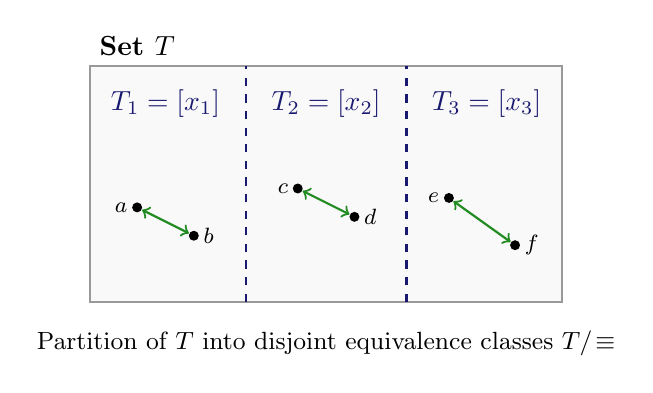
\begin{tikzpicture}[scale=1.2]
% \begin{hidden}
% - Canvas: scale=1.2, set T as an outer rectangle [0,5] x [0,2.8], divided into 3 disjoint blocks
% - Subsets: T_1 at [0,1.7], T_2 at [1.7,3.4], T_3 at [3.4,5]
% - Elements: dots inside each class representing elements related by \equiv
% - Labels: T_1, T_2, T_3 above each partition, T overall
% \end{hidden}
    % Outer bounding box T
    \draw[thick, gray!80, fill=gray!5] (0,0) rectangle (5, 2.5);
    \node[above right, font=\bfseries] at (0, 2.5) {Set $T$};

    % Vertical partition lines
    \draw[thick, dashed, MidnightBlue] (1.65, 0) -- (1.65, 2.5);
    \draw[thick, dashed, MidnightBlue] (3.35, 0) -- (3.35, 2.5);

    % Equivalence Classes
    \node[MidnightBlue, font=\bfseries] at (0.8, 2.1) {$T_1 = [x_1]$};
    \node[MidnightBlue, font=\bfseries] at (2.5, 2.1) {$T_2 = [x_2]$};
    \node[MidnightBlue, font=\bfseries] at (4.2, 2.1) {$T_3 = [x_3]$};

    % Representative dots: labels left of the first and right of the second point, away from the arrows
    \fill (0.5, 1.0) circle (1.5pt) node[left] {\footnotesize $a$};
    \fill (1.1, 0.7) circle (1.5pt) node[right] {\footnotesize $b$};
    \draw[<->, shorten <=2pt, shorten >=2pt, thick, ForestGreen] (0.5, 1.0) -- (1.1, 0.7);

    \fill (2.2, 1.2) circle (1.5pt) node[left] {\footnotesize $c$};
    \fill (2.8, 0.9) circle (1.5pt) node[right] {\footnotesize $d$};
    \draw[<->, shorten <=2pt, shorten >=2pt, thick, ForestGreen] (2.2, 1.2) -- (2.8, 0.9);

    \fill (3.8, 1.1) circle (1.5pt) node[left] {\footnotesize $e$};
    \fill (4.5, 0.6) circle (1.5pt) node[right] {\footnotesize $f$};
    \draw[<->, shorten <=2pt, shorten >=2pt, thick, ForestGreen] (3.8, 1.1) -- (4.5, 0.6);

    \node[below, font=\small] at (2.5, -0.2) {Partition of $T$ into disjoint equivalence classes $T/\!\equiv$};
\end{tikzpicture}
\end{center}
\end{content}

\subsection{The Equivalence Relation on Pairs}

\begin{speech}[00:40:21 - 00:41:03]
We have to define the equivalence relation. So, we now define this equivalence relation on our set $S$, which is the set of pairs. You should think about these pairs as numerator and denominator, but those are just words here.

We need to define: when is $(x_1, y_1)$ equivalent to $(x_2, y_2)$? We need a definition for this.

Okay, so what's the answer going to be? Yeah?
\end{speech}

\begin{student}[Student Answer]
$x_1 y_2 = x_2 y_1$.
\end{student}

\begin{speech}[00:41:06 - 00:42:06]
Very good. So, the definition is just exactly what you do with integer arithmetic: if you have a fraction, you say they're equal if $x_1 y_2 = x_2 y_1$, okay? That's the definition. There's nothing more or less than that; that's the whole definition. 

And it's motivated by the integers. It's very important for this definition that this is only about $R$, right? This whole discussion starts with $R$, so we can only say things that are about $R$. We can make these pairs --- that's only about $R$. We want to define this equivalence relation; at the end, these things are only in $R$, and the definition is only about some equation in $R$, okay? So, we haven't gotten out of $R$, in some sense, in this whole discussion. Is that clear?
\end{speech}

\begin{hidden}
% timestamp: 00:42:00
% topic: Definition of the equivalence relation on S and verification of reflexivity, symmetry, transitivity
% board_state: def:equiv-relation-S, 3 properties on board
% next_goal: Verify transitivity using the integral domain property
% open_loops: none
\end{hidden}

\begin{content}[Definition of the Equivalence Relation on \texorpdfstring{$S$}{S}]
\begin{definition}[Equivalence Relation on $S$]\label[definition]{def:equiv-relation-S}
On the set $S = \{ (x, y) \in R \times R \mid y \ne 0 \}$, we define the relation $\equiv$ by:
\begin{equation}\label{eq:equiv-relation-formula}
(x_1, y_1) \equiv (x_2, y_2) :\iff x_1 y_2 = x_2 y_1 \quad (\text{in } R).
\end{equation}
\end{definition}

\begin{steps}[Conceptual Motivation: Cross-Multiplication]
This relation is the formal algebraic counterpart to equating cross-products of fractions:
\[
\frac{x_1}{y_1} = \frac{x_2}{y_2} \iff x_1 y_2 = x_2 y_1.
\]
Crucially, formula \eqref{eq:equiv-relation-formula} involves only multiplication within the ring $R$, without invoking any external concept of division or fraction.
\end{steps}
\end{content}

\subsection{Verification of Equivalence Relation Properties}

\begin{speech}[00:42:06 - 00:44:09]
Okay, so now we come to an issue: why is this an equivalence relation? This is the question that you should have asked your teacher in first grade or whatever it was. That's like the whole question about the rational numbers, in some sense --- I mean the foundations.

\inlinemetanote{erases the lower chalkboard}

This is the first part where we have to do a little bit of algebra. 

The first two properties: $x = x$, that's just identically true, okay? That's not a problem. We have to check three properties. 

The first is if I take $(x_1, y_1)$, this is equivalent to itself \inlinemetanote{equivalent to itself}. Why is this? Because by definition, this is equal to $x_1 y_1 = x_1 y_1$, so we're very happy about that; there was nothing to do here. 

You also have to check the symmetric property: that if we have $(x_1, y_1) \equiv (x_2, y_2)$, then the other way around is fine, and it'll just be the same equation. There's nothing to check about that.
\end{speech}

\begin{speech}[00:44:09 - 00:45:00]
So, the interesting one is the transitive property. This is the only fun one to check. We start with this --- these are the inputs: $(x_1, y_1) \equiv (x_2, y_2)$ and $(x_2, y_2) \equiv (x_3, y_3)$. And we must show --- this is for us to do --- that $(x_1, y_1) \equiv (x_3, y_3)$. 

The thing that's a little funny about this is that we have to write the first equation. This is what we have, that's what we've assumed, that's in the left column. What we have...
\inlinemetanote{bell chimes}

Okay, you'll have to wait until after the break for this excitement to continue.
\end{speech}

\begin{content}[Verification of Reflexivity and Symmetry on \texorpdfstring{$S$}{S}]
\begin{proposition}[Reflexivity and Symmetry of $\equiv$]\label[proposition]{prop:equiv-refl-sym}
The relation $\equiv$ defined on $S = \{ (x, y) \in R \times R \mid y \ne 0 \}$ by:
\begin{equation}\label{eq:equiv-def-recap}
(x_1, y_1) \equiv (x_2, y_2) \iff x_1 y_2 = x_2 y_1
\end{equation}
is reflexive and symmetric.
\end{proposition}

\begin{proof}
Let $(x_1, y_1), (x_2, y_2) \in S$:
\begin{itemize}
    \item \textbf{Reflexivity:} Trivially $x_1 y_1 = x_1 y_1$, which by \eqref{eq:equiv-def-recap} immediately implies:
    \[
    (x_1, y_1) \equiv (x_1, y_1).
    \]
    \item \textbf{Symmetry:} Assume $(x_1, y_1) \equiv (x_2, y_2)$. Then $x_1 y_2 = x_2 y_1$. By symmetry of equality in $R$:
    \[
    x_2 y_1 = x_1 y_2 \implies (x_2, y_2) \equiv (x_1, y_1).
    \]
\end{itemize}
\end{proof}
\end{content}

\begin{pause}[Mid-Lecture Break]
The lecturer announces the standard mid-lecture pause. The recording resumes after the break at timestamp 00:45:05.
\end{pause}

% --- TEIL 3 ---

\begin{speech}[00:45:05 - 00:46:37]
Okay, so let's start. I should say that very few people have found my office, and it turns out I'll be in this visitor office for most of the semester, because they're clearing some kind of nuclear waste from my current office. So, my office now is HG G 65.1, if you want to find me there. \inlinemetanote{writes \qt{HG G 65.1} on the chalkboard}

And yeah, I'm afraid I'll be there for most of the semester. 

We come to this point that's actually kind of fun and interesting. We started with an integral domain, and led by the analogy with the rational numbers, we come to defining this field as some equivalence class of pairs, where --- and I should have said this, and I did say it, but I didn't write it, so the way to think about this... \inlinemetanote{writes \qt{Think of as $x_1/y_1$} on the chalkboard}

This is the mathematical text: think of it as $x_1/y_1$, or $x/y$. You think of this pair in $S$ as $x/y$, okay? Just like with the integers. But as an object, it's this formal object. 

And then there was this proposal, which is correct, on how to define the equivalence relation. And now we need to actually check something: is it an equivalence relation? We have to prove the transitive property, and so we start with: what do we have?
\end{speech}

\begin{speech}[00:46:37 - 00:48:07]
What we have is that equivalence. If we translate that into equations, it says: $x_1 y_2$ --- and we have to be very careful of the subscripts, otherwise you'll confuse yourself --- $x_1 y_2 = x_2 y_1$.

And then what we also have here is $x_2 y_3 = x_3 y_2$.

Okay, and what we want is this thing, which is $x_1 y_3 = x_3 y_1$.

The puzzling thing about this is that we have these quadratic equations and we need to get another quadratic equation. This seems a little bit unfortunate, because you might think you have to do some linear algebra with quadratic equations, and that's not going to work --- you're not going to get a new quadratic equation from these.

So, the correct answer is that we're supposed to multiply here. The clever thing is to multiply the top equation by $y_3$, which is what we want. Multiply by $y_3$, and we get $x_1 y_2 y_3 = x_2 y_1 y_3$.

Okay, so this is kind of good: we see the $x_1 y_3$ here. Can you see what we have to do next? This is actually algebra. What?
\end{speech}

\begin{student}[Student Answer]
\inlinemetanote{suggests substituting from the second equation into the first}
\end{student}

\begin{speech}[00:48:08 - 00:49:55]
Yeah, you could do that, but why don't we just take this $y_2 y_3$ here and use this equation? It's the same thing. So, we take the $y_2 y_3$ and we use this equation to flip them.

This is all about subscripts, and I should just tell you that subscripts have always been difficult for me.

Do you accept that? Because I just took this and flipped them using this equation.

So, now what do we do? We have here $x_1 y_3$, that looks pretty good, and we have $y_3 y_1$, but they're both multiplied by $y_2$, right?

Now we use the fact that in these pairs, the second one is always born non-zero; that's part of being in this set: the second one has to be non-zero.

And this is an integral domain, so then we use the integral domain property.

As I said, this is a place where it's extremely important that it's an integral domain. Since $y_2 \ne 0$, we can cancel, okay? Because being an integral domain says that's the cancellation property. Is that okay?

If $y_2$ is not zero, we can cancel it. So, we cancel it. This is kind of dramatic, but we cancel it here. \inlinemetanote{cancels $y_2$ from both sides on the chalkboard}

And that's what we want! We have now proven transitivity. And you see there was a little bit of cleverness here; it's easy to confuse yourself.
\end{speech}

\begin{hidden}
% timestamp: 00:49:50
% topic: Transitivity of the equivalence relation on S
% board_state: prop:equiv-on-S, eq:trans-hyp1, eq:trans-hyp2, cancellation via integral domain
% next_goal: Formal definition of the field of fractions F = S/~ and canonical inclusion map i: R -> F
% open_loops: none
\end{hidden}

\begin{content}[Proof of Transitivity and the Role of the Integral Domain]
\begin{proposition}[Transitivity of $\equiv$ on $S$]\label[proposition]{prop:equiv-on-S}
Let $R$ be an integral domain. The relation $\equiv$ on $S$ defined by $(x_1, y_1) \equiv (x_2, y_2) \iff x_1 y_2 = x_2 y_1$ is transitive. Consequently, $\equiv$ is an equivalence relation on $S$.
\end{proposition}

\begin{proof}
Let $(x_1, y_1), (x_2, y_2), (x_3, y_3) \in S$, which implies $y_1, y_2, y_3 \in R \setminus \{0\}$.

\textbf{1. Assumptions:}
We assume the relations:
\begin{align}
(x_1, y_1) \equiv (x_2, y_2) &\implies x_1 y_2 = x_2 y_1, \label{eq:trans-hyp1} \\
(x_2, y_2) \equiv (x_3, y_3) &\implies x_2 y_3 = x_3 y_2. \label{eq:trans-hyp2}
\end{align}

\textbf{2. Target:}
We must prove that $(x_1, y_1) \equiv (x_3, y_3)$, which means showing that:
\begin{equation}\label{eq:trans-target}
x_1 y_3 = x_3 y_1.
\end{equation}

\textbf{3. Derivation via Multiplication and Substitution:}
Multiplying equation \eqref{eq:trans-hyp1} on both sides by $y_3 \in R$:
\begin{equation}\label{eq:trans-mult}
(x_1 y_2) y_3 = (x_2 y_1) y_3 \iff (x_1 y_3) y_2 = (x_2 y_3) y_1.
\end{equation}
Substituting $x_2 y_3 = x_3 y_2$ from \eqref{eq:trans-hyp2} into the right-hand side of \eqref{eq:trans-mult}:
\begin{equation}\label{eq:trans-subst}
(x_1 y_3) y_2 = (x_3 y_2) y_1 = (x_3 y_1) y_2.
\end{equation}
Subtracting the right-hand side gives:
\begin{equation}\label{eq:trans-factored}
(x_1 y_3 - x_3 y_1) y_2 = 0.
\end{equation}

\textbf{4. Cancellation via the Integral Domain Property:}
By definition of $S$, $y_2 \ne 0$. Because $R$ is an \textbf{integral domain}, it contains no zero divisors:
\[
ab = 0 \text{ with } b \ne 0 \implies a = 0.
\]
Applying this cancellation property to \eqref{eq:trans-factored} with $b = y_2 \ne 0$:
\[
x_1 y_3 - x_3 y_1 = 0 \implies x_1 y_3 = x_3 y_1.
\]
Thus, $(x_1, y_1) \equiv (x_3, y_3)$, which completes the proof.
\end{proof}

\begin{steps}[Why Integral Domains Are Essential for Transitivity]
Notice where the ring axioms alone would fail: equation \eqref{eq:trans-factored} holds in any commutative ring. However, to deduce $x_1 y_3 = x_3 y_1$ from $(x_1 y_3 - x_3 y_1)y_2 = 0$, we must divide out and cancel the non-zero element $y_2$. If $R$ has zero divisors, the relation $\equiv$ can \emph{fail} to be transitive. For instance, in $\mathbb{Z}/6\mathbb{Z}$ (with $y_2 = \bar{2}$ and $x_1 y_3 - x_3 y_1 = \bar{3}$): $(\bar{3}, \bar{1}) \equiv (\bar{0}, \bar{2})$ since $\bar{3} \cdot \bar{2} = \bar{0} = \bar{0} \cdot \bar{1}$, and $(\bar{0}, \bar{2}) \equiv (\bar{0}, \bar{1})$ since $\bar{0} \cdot \bar{1} = \bar{0} = \bar{0} \cdot \bar{2}$, but $(\bar{3}, \bar{1}) \not\equiv (\bar{0}, \bar{1})$ since $\bar{3} \cdot \bar{1} = \bar{3} \neq \bar{0} = \bar{0} \cdot \bar{1}$.
\end{steps}
\end{content}

\subsection{Definition of the Field of Fractions and Canonical Embedding}

\begin{speech}[00:49:55 - 00:51:06]
We have come so far as to define $S$ as a set with an equivalence relation. So, now we can define the points of the field that we're constructing, which will be the equivalence classes...

\inlinemetanote{The lecturer begins erasing the lower chalkboards}

This was almost like the first piece of algebra in this class, I think. I don't remember what we did; did we have any algebra before?

By that I mean playing with equations. Which, in the end... you know, I'm saying a lot of words, but in the end the subject is about equations, that's...
\end{speech}

\begin{speech}[00:51:06 - 00:52:37]
Okay, so where are we? We started with $R$ as an integral domain. We constructed $S$ with an equivalence relation, and from this we define $F$.

The name of this is the field of fractions of $R$ --- \qt{field of fractions of $R$}, that's the name of this object. $F$ is equal to the set of equivalence classes of $S$. Is it completely clear what this thing is?

We have defined $S$, we have defined an equivalence relation, we took great pains to check all of its properties, and so we get the set of equivalence classes, and that is $F$.

Then we need to do a lot of things. But let's start by defining the map which is the inclusion from $R$ to $F$, because we said this $F$ should be a field that contains $R$. That means we have to have some way of getting points from $R$ to $F$. And what's that way going to be?

This inclusion $i$: we have to put $R$ into $F$. In other words, if I have an element $r \in R$ --- normally people don't even write it, but I just... we have to put it into $F$. That means we have to assign it an equivalence class in this set. So, what are we going to do? 

Yeah?
\end{speech}

\begin{student}[Student Answer]
$(r, 1)$?
\end{student}

\begin{speech}[00:52:39 - 00:53:41]
Yeah, that's a good idea: $(r, 1)$.

It has some advantages: $1 \ne 0$, because an integral domain is never the zero ring (Recall: \cref{def:integral-domain}). So, this is legal, this is an element of $S$, and then we can take its equivalence class.

I'm not going to write equivalence classes like $[(r, 1)]$ everywhere because it becomes too complicated. You could say formally take its equivalence class like this, but if you start doing this, you get committed to writing things like $[(3, 4)]$ for rational numbers, and no one ever does that. So, we don't want to do it, but this would be kind of more logically correct.

When I write this, it's just the equivalence class. I looked at what the book does, and the book says that $(r, 1)$ is an element of $S$, and that is its equivalence class. That's a very clever solution. I wouldn't say it's totally standard, but anyway; standard is just to ignore the issue.

So, this is the equivalence class here. Is this reasonable? Well, it better at least be... yeah...
\end{speech}

\begin{student}[Student Question]
So, the set $S$, is it the whole $R \times R$, or is it just any subset of $R \times R$?
\end{student}

\begin{speech}[00:53:50 - 00:55:47]
No, the set $S$ was very precisely defined on the previous board: $S$ is equal to those elements in $R \times R$ where $y \ne 0$. That's $S$. \inlinemetanote{writes $S = \{ (x, y) \mid x, y \in R, \ y \neq 0 \}$ on the board}

And this is an element of $S$ because $1 \ne 0$; and $1 \ne 0$ because $R$ is an integral domain, and an integral domain is by definition not the zero ring. That's the full logical certificate, if you want it.

Still, we'd like more: we'd like this to be an injection. \inlinemetanote{writes \qt{Is $i$ injective?} on the board}

This means: when are $(r, 1)$ and $(\hat{r}, 1)$ in the same equivalence class of $S$, right? \inlinemetanote{writes When are $(r, 1)$ and $(\hat{r}, 1)$ in the same equivalence class of $S$} That's what injectivity is about.

How do we check this? The answer is that these are in the same equivalence class if and only if that equivalence class identity holds: if and only if $r \cdot 1 = \hat{r} \cdot 1$, which is if and only if $r = \hat{r}$. This is great for us, because it shows that this is an injection. \inlinemetanote{writes $r \cdot 1 = \hat{r} \cdot 1 \iff r = \hat{r}$ and puts a checkmark}

We've constructed... there's a lot of things to do in this, like a big house where you have to build all the pieces of it. This shows that now we have not only defined $F$, we've defined $i$, and we've put $R$ inside $F$. And this placement is injective, okay?
\end{speech}

\begin{hidden}
% timestamp: 00:55:40
% topic: Definition of the field of fractions F = S/~ and canonical inclusion map i: R -> F
% board_state: def:field-of-fractions, def:canonical-inclusion, prop:inclusion-injective
% next_goal: Define the field operations (zero, unit, addition, multiplication) on F
% open_loops: none
\end{hidden}

\begin{content}[Definition of the Field of Fractions and Canonical Embedding]
\begin{definition}[Field of Fractions]\label[definition]{def:field-of-fractions}
Let $R$ be an integral domain, and let $S := \{ (x, y) \in R \times R \mid y \ne 0 \}$. The \newterm{field of fractions} (or quotient field) of $R$, denoted by $\operatorname{Frac}(R)$ or $F$, is defined as the quotient set:
\begin{equation}\label{eq:field-of-fractions-def}
F := S/\!\equiv \, = \{ [(x, y)] \mid (x, y) \in S \}.
\end{equation}
The equivalence class $[(x, y)]$ is commonly written as $\frac{x}{y}$.
\end{definition}

\begin{definition}[Canonical Inclusion Map]\label[definition]{def:canonical-inclusion}
We define the canonical embedding $i \colon R \to F$ by assigning to each $r \in R$ the equivalence class of the pair $(r, 1)$:
\begin{equation}\label{eq:canonical-inclusion-def}
i(r) := [(r, 1)] \in F.
\end{equation}
\end{definition}

\begin{proposition}[Injectivity of the Canonical Inclusion]\label[proposition]{prop:inclusion-injective}
The canonical map $i \colon R \to F$ is injective.
\end{proposition}

\begin{proof}
Let $r, \hat{r} \in R$. By definition of equality in the quotient set $F = S/\!\equiv$:
\begin{align*}
i(r) = i(\hat{r}) &\iff [(r, 1)] = [(\hat{r}, 1)] \\
&\iff (r, 1) \equiv (\hat{r}, 1) \\
&\iff r \cdot 1 = \hat{r} \cdot 1 \\
&\iff r = \hat{r}.
\end{align*}
Therefore, $i$ is injective.
\end{proof}

\begin{steps}[Why $1_R \ne 0_R$ Is Guaranteed]
For the pair $(r, 1)$ to belong to $S$, the denominator must satisfy $1 \ne 0$. By condition (i) of \cref{def:integral-domain}, an integral domain must satisfy $1_R \ne 0_R$ (i.e., it cannot be the trivial zero ring). Hence, $(r, 1) \in S$ is unconditionally valid for every $r \in R$.
\end{steps}
\end{content}

\subsection{Field Operations on the Field of Fractions: Zero, Unit, and Addition}

\begin{speech}[00:55:50 - 00:57:04]
As I said, this is just the beginning of the story. $R$ already is born with all of the data: $(R, +, \cdot, 0, 1)$. We need to define all the structures on $F$ and show this is a homomorphism also.
\inlinemetanote{The lecturer pushes the upper chalkboards up and erases the middle boards}
\end{speech}

\begin{speech}[00:57:04 - 00:58:39]
We have to start talking about all the structures for $F$ as a field. And for many of them, we don't have any choice: the zero in $F$ has to correspond to the zero in $R$ for it to be a homomorphism. So, the zero in $F$ has to be $(0, 1)$. \inlinemetanote{writes Zero in $F$ has to be $(0, 1)$}

And also the unit: the unit in $F$ has to be $(1, 1)$, because of course it has to correspond to the unit in $R$ by the rule of getting $R$ to $F$. \inlinemetanote{writes unit in $F$ has to be $(1, 1)$}

We don't really have any choice in this matter. But we have to define plus and multiplication on $F$. \inlinemetanote{writes We have to define $+, \cdot$ on $F$} That's something that we have to construct: we have to define it, check it's compatible with $R$, check it satisfies the field axioms --- and it's a lot of long and boring work.

The interesting part to start with is that we have to define it. If we have an element here, $(x_1, y_1) \in S$, and we have another one, $(x_2, y_2) \in S$, then we have to define this operation. This is up to us; we must define it. \inlinemetanote{writes $(x_1, y_1) + (x_2, y_2)$ with \qt{We must define} under the $+$}

That's the problem. So, what's the solution? How are we going to define this? What do you think? 

Tell me.
\end{speech}

\begin{student}[Student Answer]
Take $x_1 y_2 + x_2 y_1$, and $y_1 y_2$.
\end{student}

\begin{speech}[00:58:43 - 01:00:00]
Yeah, so we just use the standard definition for how you add fractions. \inlinemetanote{writes $(x_1 y_2 + x_2 y_1, y_1 y_2)$ on the board} Meaning you pretend that it's this problem, which it kind of is: \inlinemetanote{writes $\frac{x_1}{y_1} + \frac{x_2}{y_2} = \frac{x_1 y_2 + x_2 y_1}{y_1 y_2}$ on the right} You know how to do this.

I hope I got the subscripts right; you should tell me if I get the subscripts wrong.

This is the definition, nothing more, nothing less.

Now, is it a legal definition? There's an easy part: for it to be legal, the denominator better not be zero, because in our set $S$, the one in the basement always has to be non-zero.

We have here that this guy's non-zero, that guy's non-zero, and that implies their product is non-zero, because it is an integral domain. \inlinemetanote{draws an arrow to $y_1 y_2$ and writes \qt{non zero, $R$ is an int dom}} Is that clear? Otherwise, if this were zero, this would not be legal.
\end{speech}

\begin{speech}[01:00:00 - 01:01:45]
That's the easy part. The hard part is you have to check that... this is a definition on $S$, but we have to check that it's well-defined on equivalence classes.

That means if I trade this person for another one in the same equivalence class, and I trade this for another person in the same equivalence class, the result has to be in the same equivalence class. Is that clear?

That's the check of rational arithmetic. That's the check that I claim, to understand the rational numbers, you should have done in school. Otherwise, what are you doing? You're doing some random manipulation.

So, you have to check this. \inlinemetanote{writes \qt{You have to check the indep. of choices of equiv. class} on the board}

We've already done this kind of thing twice in the lecture. If you just do it and follow your nose, you'll see it all unwind: you just use the definition, and you have to say formally that this result respects our definition of the equivalence class.

In various books they do it; mostly it's left as an exercise. It's really important, so you should do it. If I do it, it's just a bunch of indices --- it doesn't really help. You have to go through it yourself.

Is it clear what the problem is? I recommend trying this yourself, and if you get stuck, look at the book. The book does it. It'll give you a line of things, and you can imagine it's probably true.
\end{speech}

\begin{hidden}
% timestamp: 01:01:40
% topic: Definition of zero, unit, and addition on F and well-definedness
% board_state: zero in F is (0,1), unit in F is (1,1), addition formula on F, checking non-zero denominator via integral domain
% next_goal: Define multiplication on F and prove compatibility with equivalence classes
% open_loops: none
\end{hidden}

\begin{content}[Neutral Elements and Addition on the Field of Fractions]
\begin{definition}[Neutral Elements in $F$]\label[definition]{def:neutral-elements-F}
The zero element and multiplicative unit in $F$ are defined by:
\begin{align}
0_F &:= i(0_R) = [(0, 1)], \label{eq:zero-F} \\
1_F &:= i(1_R) = [(1, 1)]. \label{eq:unit-F}
\end{align}
\end{definition}

\begin{definition}[Addition on $F$]\label[definition]{def:addition-F}
For any two equivalence classes $[(x_1, y_1)]$, $[(x_2, y_2)] \in F$, addition is defined by:
\begin{equation}\label{eq:addition-F-formula}
[(x_1, y_1)] + [(x_2, y_2)] := [(x_1 y_2 + x_2 y_1, y_1 y_2)].
\end{equation}
\end{definition}

\begin{proposition}[Legitimacy and Well-Definedness of Addition]\label[proposition]{prop:addition-well-defined}
Addition on $F$ as given in \eqref{eq:addition-F-formula} is well-defined.
\end{proposition}

\begin{proof}
We verify two essential requirements:
\begin{enumerate}[label=\textbf{(\arabic*)}]
    \item \textbf{Legitimacy of the Denominator:} For $(x_1 y_2 + x_2 y_1, y_1 y_2)$ to lie in $S$, we must have $y_1 y_2 \ne 0$. Since $(x_1, y_1), (x_2, y_2) \in S$, we know $y_1 \ne 0$ and $y_2 \ne 0$. Because $R$ is an \textbf{integral domain}, the product of two non-zero elements is non-zero:
    \[
    y_1 \ne 0 \land y_2 \ne 0 \implies y_1 y_2 \ne 0.
    \]
    Thus, $(x_1 y_2 + x_2 y_1, y_1 y_2) \in S$.
    
    \item \textbf{Independence of Representatives:} Suppose $(x_1, y_1) \equiv (\hat{x}_1, \hat{y}_1)$ and $(x_2, y_2) \equiv (\hat{x}_2, \hat{y}_2)$, meaning:
    \begin{equation}\label{eq:add-well-def-hyp}
    x_1 \hat{y}_1 = \hat{x}_1 y_1 \quad \text{and} \quad x_2 \hat{y}_2 = \hat{x}_2 y_2.
    \end{equation}
    We must show that $(x_1 y_2 + x_2 y_1, y_1 y_2) \equiv (\hat{x}_1 \hat{y}_2 + \hat{x}_2 \hat{y}_1, \hat{y}_1 \hat{y}_2)$, which requires:
    \[
    (x_1 y_2 + x_2 y_1)(\hat{y}_1 \hat{y}_2) \overset{?}{=} (\hat{x}_1 \hat{y}_2 + \hat{x}_2 \hat{y}_1)(y_1 y_2).
    \]
    Expanding the left-hand side and applying \eqref{eq:add-well-def-hyp}:
    \begin{align*}
    (x_1 y_2 + x_2 y_1)\hat{y}_1 \hat{y}_2 &= (x_1 \hat{y}_1)(y_2 \hat{y}_2) + (x_2 \hat{y}_2)(y_1 \hat{y}_1) \\
    &= (\hat{x}_1 y_1)(y_2 \hat{y}_2) + (\hat{x}_2 y_2)(y_1 \hat{y}_1) \\
    &= (\hat{x}_1 \hat{y}_2 + \hat{x}_2 \hat{y}_1)y_1 y_2.
    \end{align*}
    This establishes equivalence, confirming that addition is independent of the choice of representative.
\end{enumerate}
\end{proof}
\end{content}

\subsection{Multiplication and Ring Embedding Properties}

\begin{speech}[01:01:45 - 01:03:17]
\inlinemetanote{The lecturer erases the left chalkboard}

You also have to do it with multiplication. Multiplication is a bit easier; addition is the most painful one. Also define multiplication:
\[
(x_1, y_1) \cdot (x_2, y_2) = (x_1 x_2, y_1 y_2),
\]
which will surprise no one, okay? \inlinemetanote{writes Also define $\cdot$: $(x_1, y_1) \cdot (x_2, y_2) \overset{\text{def}}{=} (x_1 x_2, y_1 y_2)$} That's the definition, right?

And again, next is the check of compatibility with the equivalence classes. This check is easy, so I'll do it since it's easy.
\end{speech}

\begin{speech}[01:03:17 - 01:05:40]
Suppose we have that $(x_1, y_1)$ is in the same equivalence class as $(\hat{x}_1, \hat{y}_1)$, and $(x_2, y_2)$ is in the same equivalence class as $(\hat{x}_2, \hat{y}_2)$. \inlinemetanote{writes $(x_1, y_1) \equiv (\hat{x}_1, \hat{y}_1)$, $(x_2, y_2) \equiv (\hat{x}_2, \hat{y}_2)$}

Then we have to show --- that's the input, right? --- we must show that $(x_1 x_2, y_1 y_2)$ is in the same equivalence class as if we chose the other representatives: $(\hat{x}_1 \hat{x}_2, \hat{y}_1 \hat{y}_2)$. \inlinemetanote{writes We must show $(x_1 x_2, y_1 y_2) \equiv (\hat{x}_1 \hat{x}_2, \hat{y}_1 \hat{y}_2)$} That's what we have to do.

What we know is this: the equation that these are in the same equivalence class is $x_1 \hat{y}_1 = \hat{x}_1 y_1$, and this equation is $x_2 \hat{y}_2 = \hat{x}_2 y_2$, all very confusing. \inlinemetanote{writes $x_1 \hat{y}_1 = \hat{x}_1 y_1$, $x_2 \hat{y}_2 = \hat{x}_2 y_2$}

And now we just multiply them together! These are what we know, and then we have these two equations: we can multiply them all together, and we get $x_1 x_2 \hat{y}_1 \hat{y}_2 = \hat{x}_1 \hat{x}_2 y_1 y_2$. \inlinemetanote{writes $\implies x_1 x_2 \hat{y}_1 \hat{y}_2 = \hat{x}_1 \hat{x}_2 y_1 y_2$}

That equation is exactly the certificate that these things are in the same equivalence class, okay? This implies that.

This shows that if I pick different equivalence classes here, the result doesn't matter. This one I did completely, because it's easy: all you do is multiply. For the other one, you have to do the kind of tricks we were doing before, where you have to clear the denominators, etc., so you can do that, so to speak, on your own time.
\end{speech}

\begin{speech}[01:05:40 - 01:06:50]
Then you have to check that these definitions are compatible with $R$. I mean, they're just all defined that way, meaning we have to check that this inclusion $i$ is a homomorphism of rings. \inlinemetanote{writes Check $i \colon R \to F$ is a hom of rings}

And again, there's really nothing to this: it means that if you take $r + \hat{r}$, and then you go by $i$, you get $(r + \hat{r}, 1)$. \inlinemetanote{writes $r + \hat{r} \xrightarrow{i} (r + \hat{r}, 1)$ and below it $= (r, 1) + (\hat{r}, 1)$}

Then you have to check that this thing is equal to $(r, 1) + (\hat{r}, 1)$, and that's the same by the definition that we used there. But you have to check it, and you have to also check it for multiplication. So, it's just a bunch of checking. Here, all the cards are played, and you just have to check everything, okay?
\end{speech}

\begin{hidden}
% timestamp: 01:06:40
% topic: Multiplication on F, verification of well-definedness, and homomorphism properties of i: R -> F
% board_state: def:mult-F, prop:mult-well-defined, thm:field-of-fractions-properties
% next_goal: Summary of the complete construction of the field of fractions
% open_loops: none
\end{hidden}

\begin{content}[Multiplication on $F$ and Ring Homomorphism Properties]
\begin{definition}[Multiplication on $F$]\label[definition]{def:multiplication-F}
For any $[(x_1, y_1)], [(x_2, y_2)] \in F$, multiplication is defined by:
\begin{equation}\label{eq:multiplication-F-formula}
[(x_1, y_1)] \cdot [(x_2, y_2)] := [(x_1 x_2, y_1 y_2)].
\end{equation}
\end{definition}

\begin{proposition}[Well-Definedness of Multiplication]\label[proposition]{prop:mult-well-defined}
Multiplication on $F$ is well-defined and independent of the choice of representative.
\end{proposition}

\begin{proof}
The pair $(x_1 x_2, y_1 y_2)$ lies in $S$, since $y_1 y_2 \neq 0$ in the integral domain $R$ (as for addition, \cref{prop:addition-well-defined}).

Let $(x_1, y_1) \equiv (\hat{x}_1, \hat{y}_1)$ and $(x_2, y_2) \equiv (\hat{x}_2, \hat{y}_2)$ in $S$. By definition of $\equiv$:
\begin{equation}\label{eq:mult-hyp}
x_1 \hat{y}_1 = \hat{x}_1 y_1 \quad \text{and} \quad x_2 \hat{y}_2 = \hat{x}_2 y_2.
\end{equation}
Multiplying these two equations in the commutative ring $R$:
\[
(x_1 \hat{y}_1)(x_2 \hat{y}_2) = (\hat{x}_1 y_1)(\hat{x}_2 y_2) \implies (x_1 x_2)(\hat{y}_1 \hat{y}_2) = (\hat{x}_1 \hat{x}_2)(y_1 y_2).
\]
By \eqref{eq:equiv-def-recap}, this algebraic identity is precisely the condition for equivalence:
\[
(x_1 x_2, y_1 y_2) \equiv (\hat{x}_1 \hat{x}_2, \hat{y}_1 \hat{y}_2).
\]
Thus, $[(x_1 x_2, y_1 y_2)] = [(\hat{x}_1 \hat{x}_2, \hat{y}_1 \hat{y}_2)]$, proving well-definedness.
\end{proof}

\begin{proposition}[$i$ is an Injective Ring Homomorphism]\label[proposition]{prop:i-is-homomorphism}
The canonical inclusion $i \colon R \hookrightarrow F$ is an injective ring homomorphism:
\begin{align}
i(r + \hat{r}) &= i(r) + i(\hat{r}), \label{eq:i-add} \\
i(r \cdot \hat{r}) &= i(r) \cdot i(\hat{r}), \label{eq:i-mult} \\
i(1_R) &= 1_F. \label{eq:i-unit}
\end{align}
\end{proposition}

\begin{proof}
Evaluating the definitions directly:
\begin{itemize}
    \item \textbf{Additivity:}
    \[
    i(r) + i(\hat{r}) = [(r, 1)] + [(\hat{r}, 1)] = [(r \cdot 1 + \hat{r} \cdot 1, 1 \cdot 1)] = [(r + \hat{r}, 1)] = i(r + \hat{r}).
    \]
    \item \textbf{Multiplicativity:}
    \[
    i(r) \cdot i(\hat{r}) = [(r, 1)] \cdot [(\hat{r}, 1)] = [(r \hat{r}, 1 \cdot 1)] = [(r \hat{r}, 1)] = i(r \hat{r}).
    \]
    \item \textbf{Identity:}
    \[
    i(1_R) = [(1, 1)] = 1_F.
    \]
\end{itemize}
Injectivity was already established in \cref{prop:inclusion-injective}.
\end{proof}

\begin{steps}[Multiplicative Inverses in $F$]
To confirm that $F$ is indeed a field, let $[(x, y)] \in F$ with $[(x, y)] \ne 0_F = [(0, 1)]$. Then $(x, y) \not\equiv (0, 1) \implies x \cdot 1 \ne 0 \cdot y \implies x \ne 0$. Thus, $(y, x) \in S$, and:
\[
[(x, y)] \cdot [(y, x)] = [(xy, yx)] = [(1, 1)] = 1_F.
\]
Therefore, every non-zero element in $F$ possesses a multiplicative inverse $[(x, y)]^{-1} = [(y, x)]$.
\end{steps}
\end{content}

\subsection{Summary of the Explicit Construction}

\begin{speech}[01:06:50 - 01:08:46]
That is the construction. 

As I said, when you understand it, you'll realize that actually you knew the whole thing anyway in your understanding of the rational numbers. You were subconsciously doing all of this --- not explicitly, but underneath the surface, you were assuming all of these properties were true; it made rational number arithmetic work. 

There are different ways to try to learn this material, but the way that's foundational is that you actually go yourself and check all the things that you're supposed to check. That takes a little bit of time, and it's somewhat painful, but you only have to do it once in your life. 

You can read the book, too. I think that doesn't help so much, because then you just read what the author has written, and it's just a bunch of things with equalities. You can convince yourself of anything if you read what someone else did. So, the best thing is to go through all of it yourself; then you'll understand it once in your life. 

And that's the construction, so we're done with this construction. I'll just summarize here: \inlinemetanote{writes on the lower left chalkboard: \qt{Construction}, \qt{Start with $R$ int domain}, \qt{Construct $F$ = field of fractions}, $R \hookrightarrow F$, $r \to (r, 1)$}

We start with $R$ as an integral domain, and then we construct explicitly --- that's as explicit a mathematical construction as you get. You just take $R$, and you make some sets and equivalence classes and relations; it's totally explicit. We construct this $F$, which is the field of fractions. 

And $R$ sits inside $F$ by this map: $r \mapsto (r, 1)$.
\end{speech}

\begin{content}[Summary of the Construction of the Field of Fractions]
\begin{theorem}[Existence and Structure of the Field of Fractions]\label[theorem]{thm:field-of-fractions-summary}
Let $R$ be an integral domain. There exists a field $F$, called the \newterm{field of fractions} of $R$ (denoted $\operatorname{Frac}(R)$), and an injective ring homomorphism:
\[
i \colon R \hookrightarrow F, \quad r \mapsto [(r, 1)],
\]
such that:
\begin{enumerate}[label=\textbf{(\arabic*)}]
    \item \textbf{Field Structure:} $F$ is a field with zero $0_F = [(0, 1)]$ and multiplicative identity $1_F = [(1, 1)]$.
    \item \textbf{Quotient Representation:} Every element of $F$ can be written as a quotient of elements in the image of $R$:
    \begin{equation}\label{eq:frac-quotient-representation}
    \forall q \in F \ \exists r, s \in R \ (s \ne 0) \quad \text{such that} \quad q = i(r) \cdot i(s)^{-1} = \frac{i(r)}{i(s)}.
    \end{equation}
\end{enumerate}
\end{theorem}
\end{content}

% --- TEIL 4 ---

\subsection{Algebraic Perspective: Fractions in an Integral Domain}

\begin{speech}[01:08:46 - 01:09:44]
When you get used to it, the way an algebraist always thinks about this is: you have elements in $R$, and the elements of $F$ are just $r/s$; you just view them as fractions in $R$. 

This is a perfectly reasonable way to think about it. In our language, when someone writes this, what they really mean is the equivalence class of $(r, s)$ in this set $S$. That's what it actually means. And it's only legal if the bottom one is not zero, which means you're not allowed to write this anyway if the bottom one's not zero. Then you can add fractions and multiply fractions just as you would normally do, and they correspond exactly to the rules that were prescribed here. That's the natural way to think about it. 

Once all of this is done, then you just start using it like you normally would anyway. But this is the underlying foundation. 

Are there any conceptual questions about that?
\end{speech}

\begin{content}[Algebraic View: Working with Fractions]
In mathematical practice, once the formal construction of $F = S/\!\equiv$ is established, we identify $R$ with its image $i(R) \subseteq F$ and adopt standard fraction notation:
\begin{equation}\label{eq:fraction-notation-standard}
\frac{r}{s} := [(r, s)] \in \operatorname{Frac}(R) \quad (r, s \in R, \ s \ne 0).
\end{equation}

\textbf{Arithmetic in the Field of Fractions:}
Under this notation, the field operations on $\operatorname{Frac}(R)$ take the standard form familiar from elementary arithmetic:
\begin{align}
\text{Equality:} && \frac{r_1}{s_1} &= \frac{r_2}{s_2} \iff r_1 s_2 = r_2 s_1, \label{eq:frac-eq} \\
\text{Addition:} && \frac{r_1}{s_1} + \frac{r_2}{s_2} &= \frac{r_1 s_2 + r_2 s_1}{s_1 s_2}, \label{eq:frac-add} \\
\text{Multiplication:} && \frac{r_1}{s_1} \cdot \frac{r_2}{s_2} &= \frac{r_1 r_2}{s_1 s_2}, \label{eq:frac-mult} \\
\text{Inverse:} && \left(\frac{r}{s}\right)^{-1} &= \frac{s}{r} \quad (\text{provided } r \ne 0). \label{eq:frac-inv}
\end{align}
\end{content}

\section{Examples of Fields of Fractions}

\subsection{The Rationals, Gaussian Rationals, and Subrings of \texorpdfstring{$\mathbb{Q}$}{Q}}

\begin{speech}[01:09:44 - 01:10:44]
If I take $\mathbb{Z}$, you can ask: what is the field of fractions? 

The answer is going to be $\mathbb{Q}$, which means that if you start with $\mathbb{Z}$ and you do this crazy construction, you get the rational numbers. I hope that's clear by now. 

All right, so what happens if I do something else? What happens if I start with the ring of Gaussian integers? What is the field of fractions? 

That's a strange question, because I've just explained what the field of fractions is: you take the Gaussian integers, you do this construction, and that's the field of fractions. So, when I say \qt{what is the field of fractions}, what the question is actually asking is: what's another way of thinking about the answer? 

Do you have a proposal for what that is? 

Yeah?
\end{speech}

\begin{student}[Student Answer]
Just $\mathbb{Q}$ adjoined with $i$.
\end{student}

\begin{hidden}
% timestamp: 01:10:45
% topic: Field of fractions examples: Z, Z[i], Z[1/3]
% board_state: Frac(Z) = Q, Frac(Z[i]) = Q(i), Frac(Z[1/3]) = Q
% next_goal: Discuss subrings of Q and field of fractions of a field
% open_loops: none
\end{hidden}

\begin{speech}[01:10:46 - 01:12:32]
Yeah, so the answer is this: $\mathbb{Q}(i)$, which is equal to the set of $a + bi$, where $a, b \in \mathbb{Q}$. 

It's correct, but now to check this is correct, you have to do a bunch of things: one is you have to show this is a field (you can invert), and then you have to show that this sits inside, and everything here is a ratio of that. It's all true, but that's the answer here, and it requires some checking. All right, this is correct. 

What about this? We saw last week that there are some funny rings that sit inside $\mathbb{Z}$ and $\mathbb{Q}$. This ring is the set of $a/3^b$, where $a \in \mathbb{Z}$ and $b$ is some integer greater than or equal to $0$, right? We discussed this last week (Recall: \cref{ex:dyadic-rationals-subring}): the subrings that sit in between. I hope you remember. 

Do you remember? 

This is an integral domain also, because it sits inside $\mathbb{Q}$. So, what is the field of fractions of... I just gave it a name, $\mathbb{Z}[1/3]$, because you're allowed to have threes in the bottom. There are two standard names for this: one is $\mathbb{Z}[1/3]$, and the other is... yeah, that's a better name, okay. 

What is the field of fractions of this integral domain?
\end{speech}

\begin{student}[Student Answer]
Also $\mathbb{Q}$.
\end{student}

\begin{speech}[01:12:34 - 01:13:33]
Also $\mathbb{Q}$! Nothing says it can't be $\mathbb{Q}$. It certainly sits inside $\mathbb{Q}$, and everything in $\mathbb{Q}$ is already a ratio of numbers here. So, it's just $\mathbb{Q}$. If you go through this definition, you get $\mathbb{Q}$. 

As I said, you think about this field of fractions as the smallest field that contains the integral domain. You can't really contain something smaller than $\mathbb{Q}$, because it already has $\mathbb{Z}$ in it, and $\mathbb{Z}$ already gives you everything in $\mathbb{Q}$. 

So, what is the field of fractions of this? The answer is also $\mathbb{Q}$. 

In fact, if you take any ring, any integral domain that sits in between $\mathbb{Z}$ and $\mathbb{Q}$, the field of fractions is just $\mathbb{Q}$.
\end{speech}

\begin{content}[Examples: Fractions of the Integers, Gaussian Integers, and Subrings of \texorpdfstring{$\mathbb{Q}$}{Q}]
\begin{example}[The Integers]\label[example]{ex:frac-integers}
For the ring of integers $\mathbb{Z}$:
\[
\operatorname{Frac}(\mathbb{Z}) = \mathbb{Q}.
\]
\end{example}

\begin{example}[The Gaussian Integers]\label[example]{ex:frac-gaussian-integers}
For the ring of Gaussian integers $\mathbb{Z}[i] = \{ a + bi \mid a, b \in \mathbb{Z} \}$:
\[
\operatorname{Frac}(\mathbb{Z}[i]) = \mathbb{Q}(i) := \{ a + bi \mid a, b \in \mathbb{Q} \}.
\]
The field $\mathbb{Q}(i)$ is called the field of \newterm{Gaussian rationals}.
\end{example}

\begin{example}[Triadic Rationals]\label[example]{ex:frac-triadic}
Consider the ring of triadic fractions $\mathbb{Z}[\frac{1}{3}]$ (the case $m = 3$ of \cref{ex:dyadic-rationals-subring}), defined by:
\[
\mathbb{Z}\left[\frac{1}{3}\right] := \left\{ \frac{a}{3^b} \;\middle|\; a \in \mathbb{Z}, \ b \in \mathbb{Z}_{\ge 0} \right\} \subset \mathbb{Q}.
\]
Since $\mathbb{Z} \subset \mathbb{Z}[\frac{1}{3}] \subset \mathbb{Q}$, any fraction of elements from $\mathbb{Z}[\frac{1}{3}]$ is already a rational number, and every rational number $\frac{p}{q}$ can be written as a quotient of elements in $\mathbb{Z} \subset \mathbb{Z}[\frac{1}{3}]$. Thus:
\[
\operatorname{Frac}\left(\mathbb{Z}\left[\frac{1}{3}\right]\right) = \mathbb{Q}.
\]
\end{example}

\begin{proposition}[Intermediate Subrings of $\mathbb{Q}$]\label[proposition]{prop:subrings-q-frac}
Let $R$ be any subring of $\mathbb{Q}$ with $\mathbb{Z} \subseteq R \subseteq \mathbb{Q}$. Then:
\begin{equation}\label{eq:intermediate-frac-q}
\operatorname{Frac}(R) = \mathbb{Q}.
\end{equation}
\end{proposition}

\begin{center}
\begin{tikzpicture}[scale=1.3, >=Stealth]
% \begin{hidden}
% - Canvas: scale=1.3, vertical tower of inclusions: Z at (0,0), Z[1/3] at (0,1.3), Q at (0,2.6)
% - Right side: Frac map arrows from Z, Z[1/3], and Q all pointing to Q at (3.5, 1.3)
% - Colors: MidnightBlue for rings, BrickRed for fields, ForestGreen for arrows
% \end{hidden}
    % Ring Tower on Left
    \node[MidnightBlue, font=\bfseries] (Z) at (0, 0) {$\mathbb{Z}$};
    \node[MidnightBlue, font=\bfseries] (Z3) at (0, 1.3) {$\mathbb{Z}[\frac{1}{3}]$};
    \node[BrickRed, font=\bfseries] (Qleft) at (0, 2.6) {$\mathbb{Q}$};

    \draw[right hook->, thick, MidnightBlue] (Z) -- (Z3);
    \draw[right hook->, thick, MidnightBlue] (Z3) -- (Qleft);

    % Common Field of Fractions on Right
    \node[draw=BrickRed, fill=BrickRed!10, rounded corners, inner sep=6pt, font=\bfseries] (Qtarget) at (3.5, 1.3) {$\operatorname{Frac} = \mathbb{Q}$};

    \draw[->, thick, ForestGreen] (Z.east) to[bend right=20] node[midway, below, sloped, font=\footnotesize] {$\operatorname{Frac}$} (Qtarget.south west);
    \draw[->, thick, ForestGreen] (Z3.east) -- node[midway, above, font=\footnotesize] {$\operatorname{Frac}$} (Qtarget.west);
    \draw[->, thick, ForestGreen] (Qleft.east) to[bend left=20] node[midway, above, sloped, font=\footnotesize] {$\operatorname{Frac}$} (Qtarget.north west);
\end{tikzpicture}
\end{center}

\begin{steps}[Why All Intermediate Subrings Yield $\mathbb{Q}$]
By categorical minimality, $\operatorname{Frac}(R)$ is the smallest field containing $R$. Since $\mathbb{Z} \subseteq R$, any field containing $R$ must contain $\mathbb{Z}$, and hence must contain a copy of $\operatorname{Frac}(\mathbb{Z}) = \mathbb{Q}$ (\cref{thm:universal-property-q}). Since $R \subseteq \mathbb{Q}$, $\mathbb{Q}$ is already a field containing $R$. Therefore, $\operatorname{Frac}(R)$ cannot be strictly larger or smaller than $\mathbb{Q}$, forcing $\operatorname{Frac}(R) = \mathbb{Q}$.
\end{steps}
\end{content}

\subsection{Field of Fractions of an Existing Field}

\begin{speech}[01:13:33 - 01:14:49]
Okay, so now a stranger question is: what happens if... well, yeah. 

You know, on the business of guessing: once I was at a conference, and the conference had some math researchers and some high school teachers. At dinner I was sitting next to some teachers, and I was trying to explain to them my theory of how you should teach children math. And the outcome was that they wanted me disbarred from academics. 

The theory, by the way, was that on exams you should make the kids just guess the answers: no calculation, just guess everything. That's, you know, maybe a little excessive, but you know... 

Maybe a compromise: on half the exam they should just guess everything. But I think that would be really, somehow, more in the spirit of mathematics than...
\end{speech}

\begin{speech}[01:14:49 - 01:15:25]
A kind of stranger question is: suppose I start with a field. Suppose $R$ is a field. \inlinemetanote{writes Suppose $R$ is field}

Then, of course, it's still an integral domain, because every field is an integral domain (Recall: \cref{ex:fields-are-domains}). Then what is the field of fractions? \inlinemetanote{writes $R$ is int domain, $\implies$ What is the field of fraction?}

What do you think the field of fractions is going to be here? 

Yeah?
\end{speech}

\begin{student}[Student Answer]
It's $R$ itself.
\end{student}

\begin{speech}[01:15:28 - 01:16:00]
Yes, $R$ itself! \inlinemetanote{writes \qt{$R$ itself} on the board}

And the answer is $R$ itself. 

To prove that: again, this fits in with this view that it's the smallest field. If it's already a field, how could there be a smaller field that contains it? It's already a field. 

To prove it, you have to go through this construction and show that in the case where $R$ is a field, that construction just reconstructs $R$. To do that, you have to go through that construction and see it, so that's also an exercise for you. 

Those are really the basic facts.
\end{speech}

\begin{hidden}
% timestamp: 01:15:55
% topic: Field of fractions of a field is the field itself
% board_state: R is a field -> Frac(R) = R itself
% next_goal: Begin discussion of polynomial rings R[x]
% open_loops: none
\end{hidden}

\begin{content}
\begin{proposition}[Field of Fractions of a Field]\label[proposition]{prop:frac-of-a-field}
Let $K$ be a field. Then the canonical inclusion $i \colon K \hookrightarrow \operatorname{Frac}(K)$ is an isomorphism of fields:
\begin{equation}\label{eq:frac-field-itself}
\operatorname{Frac}(K) \cong K.
\end{equation}
\end{proposition}

\begin{proof}
By \cref{prop:i-is-homomorphism}, $i \colon K \hookrightarrow \operatorname{Frac}(K)$ is an injective field homomorphism. To establish surjectivity, let $[(x, y)] \in \operatorname{Frac}(K)$ with $x, y \in K$ and $y \ne 0$.
Since $K$ is a field, $y$ has a multiplicative inverse $y^{-1} \in K$. Then:
\[
(x, y) \equiv (x y^{-1}, 1) \iff x \cdot 1 = (x y^{-1}) \cdot y = x.
\]
Consequently:
\[
[(x, y)] = [(x y^{-1}, 1)] = i(x y^{-1}).
\]
Every element of $\operatorname{Frac}(K)$ is the image of the element $x y^{-1} \in K$. Hence, $i$ is surjective and constitutes a field isomorphism.
\end{proof}
\end{content}

\section{Polynomial Rings and Power Series Rings}

\subsection{Definition of the Polynomial Ring in One Indeterminate}

\begin{speech}[01:16:00 - 01:18:16]
The next topic this week is about polynomial rings. These are really fun. We'll talk about polynomial rings \inlinemetanote{writes \qt{Polynomials rings, Power series rings}}, and in some sense even more fun than polynomial rings are power series rings. 

Again, this material, in some sense, you've been using all of this already in the first year, but here we take a formal approach. 

The idea is: if I take $R$ as a ring --- and now, no assumptions, meaning not necessarily an integral domain, so this just means commutative for us: a commutative ring with unit. That's our basic ring: when we say ring with no assumptions, we mean a commutative ring with unit (Recall: \cref{rem:ring-convention}). In particular, for everything today so far, $R$ was an integral domain. Now, I don't care if it's an integral domain; it's just a commutative ring with unit. 

Then I can make a new ring here: $R[x]$. 

Here, $x$ is the variable, or sometimes it's called the indeterminate. That's kind of a fancy name, but it's just $x$, right? The indeterminate or the variable. 

The name of this ring is the polynomial ring with coefficients in $R$. Or if you want to be even more precise: the polynomial ring in one variable with coefficients in $R$. That's kind of a long sentence, but if you meet a mathematician and say, \qt{I'm going to consider the polynomial ring in one variable with coefficients in $R$}, as long as you agree on what a ring is, that's absolutely unambiguous --- the person will know exactly what you're talking about. 

What is this? Well, I have to tell you what it is as a set. So, the first thing is: what's the set?
\end{speech}

\begin{speech}[01:18:16 - 01:20:17]
Here the definition is that it's the set of polynomials in $x$ with coefficients in $R$. Polynomials look like this: $a_0 + a_1 x + a_2 x^2 + \dots$ \inlinemetanote{writes $R[x] = \{ a_0 + a_1 x + a_2 x^2 + \dots + a_n x^n \mid a_i \in R, n \ge 0 \}$ on the board}

It's these symbols, up to eventually... One of the properties of a polynomial is that it's not infinite; a polynomial is finite. That's always part of the definition in mathematics of a polynomial. That means we stop somewhere, at some $n$, with $a_n x^n$. The elements of this ring are such symbols: formal combinations of $a_i x^i$, where these $a_i$ are in $R$, and possibly different $n$, where $n \in \mathbb{Z}_{\ge 0}$. 

If I have $\mathbb{Z}[x]$, the elements in here are sometimes written $f(x)$, because we like to write polynomials with the variable. It could be, for example, $f(x) = 3 + 2x + 15x^2 + 345x^{200}$. This is a totally legitimate element of it. Other times, you'll see people just write this as $f$ and suppress the variable. Those are two different ways you can write polynomials. 

For $R[x]$, it's just the same thing: you write an element here, $f(x)$, by picking some finite number of elements of $R$ --- the coefficients, all the way to $a_n$ --- and then you just put the powers of $x$ here. 

Here, $x$ is a formal variable: there's no relation; $x$ is in some sense just a placeholder. Those are the elements of $R[x]$.
\end{speech}

\begin{speech}[01:20:17 - 01:21:26]
$R[x]$ has a confusing element, just like the integers: there's a confusing polynomial, like the constant polynomial. If I put $17$ here, that is also in $R[x]$. 

That's the polynomial that only has a constant term; it just happens that there's no $x$ in that. It's weird to write this polynomial as a function of $x$, but it is a function of $x$ --- it's a constant function. In this ring, there are also the constant polynomials, the ones with no $x$. 

Is it clear what this set is? You take $R$, and then you take an $x$ that has nothing to do with $R$ --- it's just some kind of Platonic ideal indeterminate --- and then you consider these formal linear combinations. That's what a polynomial is. 

In particular, I don't really mean anything by this plus: it's just a formal linear combination. Some authors don't like to write this because they think you might think that this plus here means something, which is a legitimate thing to think, actually.
\end{speech}

\begin{content}[{The Polynomial Ring \texorpdfstring{$R[x]$}{R[x]}: Informal Formulation}]
\recap{Polynomial rings were already used informally: $\mathbb{Z}[x] \subseteq \mathbb{Q}[x] \subseteq \mathbb{R}[x] \subseteq \mathbb{C}[x]$ in Week~1 (\cref{ex:inclusions-standard-rings}) and $\mathbb{Z}[x^2] \subset \mathbb{Z}[x]$ in Week~2 (\cref{ex:even-polynomials-subring}). Here they are defined formally.}

\begin{definition}[Polynomial Ring over a Commutative Ring]\label[definition]{def:poly-ring-informal}
Let $R$ be a commutative ring with unit $1_R$. The \newterm{polynomial ring in one variable} (or indeterminate) $x$ with coefficients in $R$, denoted $R[x]$, is defined as the set of formal expressions:
\begin{equation}\label{eq:poly-set-def}
R[x] := \left\{ \sum_{i=0}^n a_i x^i = a_0 + a_1 x + a_2 x^2 + \dots + a_n x^n \;\middle|\; n \in \mathbb{N}_0, \ a_i \in R \right\}.
\end{equation}
\end{definition}

\begin{example}[{Polynomials in $\mathbb{Z}[x]$}]\label[example]{ex:poly-zx}
In the ring $\mathbb{Z}[x]$, an element may be denoted $f(x)$ or simply $f$:
\[
f(x) = 3 + 2x + 15x^2 + 345x^{200} \in \mathbb{Z}[x].
\]
Constant elements such as $17 \in \mathbb{Z}$ correspond to polynomials of degree $0$ with $n = 0$:
\[
17 = 17 \cdot x^0 \in \mathbb{Z}[x].
\]
\end{example}

\begin{steps}[The Indeterminate as a Formal Placeholder]
Crucially, $x$ is not an element of $R$, nor does it represent an unknown numerical value in this context. It is an \newterm{indeterminate} (formal variable) acting as a positional placeholder. The symbols $+$ and $x^i$ in \eqref{eq:poly-set-def} are purely typographical markers separating the coefficients $a_i \in R$, rather than evaluations of operations.
\end{steps}
\end{content}

\subsection{Rigorous Foundation: Polynomials as Almost-Zero Sequences}

\begin{speech}[01:21:26 - 01:22:28]
\inlinemetanote{The lecturer pushes the upper chalkboard up and begins erasing the lower board}
If you look at books where they're really formally correct, they will do some weird things just so you don't get confused. I will explain it for a moment, but I don't usually do that because I think it's a little dishonest. 

When I give these lectures, I try to actually give the lectures in the way I think about the subject. There's some kind of underlying honesty in the lecture. 

If I were to be dishonest and formally correct, the way you define these polynomials is the following way.
\end{speech}

\begin{speech}[01:22:28 - 01:24:00]
You say a polynomial, an element of $R[x]$, is a tuple of elements of $R$, $(a_0, a_1, a_2, \dots)$ --- an infinite tuple --- such that there exists some $N$ such that for all $m > N$, the element in this tuple is zero, okay? \inlinemetanote{writes \qt{an element of $R[x]$ is a tuple of elements of $R$} $(a_0, a_1, a_2, \dots)$ such that $\exists N \ \forall m > N, a_m = 0$}

That's a formal definition of a polynomial in one variable, where I just give you the coefficients. The coefficients are $a_0, a_1, a_2, \dots$; they're all elements of $R$. 

I just give you the coefficients, and there could be lots of them --- any finite number --- but eventually this sequence of coefficients is all zero. That's the formal definition of a polynomial. 

It's actually the same thing that I'm saying, but it's much more reasonable to think about it with the $x$'s. This way is just so that you don't get confused formally. 

That's the set. I hope there's no confusion about the set.
\end{speech}

\begin{hidden}
% timestamp: 01:23:55
% topic: Formal definition of R[x] as sequences with finite support (almost-zero tuples)
% board_state: R[x] as infinite tuple (a_0, a_1, ...) with a_m = 0 for m > N
% next_goal: Identification of the indeterminate x as (0, 1, 0, 0, ...)
% open_loops: none
\end{hidden}

\begin{speech}[01:24:00 - 01:24:24]
In this abstract way, what is the variable $x$? \inlinemetanote{pause}

You have five minutes to figure it out. 

What's the variable $x$? In my notation there's an $x$; here there's no $x$. So, what's $x$ here? 

Yeah?
\end{speech}

\begin{student}[Student Answer]
$(0, 1, 0, \dots)$
\end{student}

\begin{speech}[01:24:27 - 01:24:40]
Yeah. So, $x$ is $(0, 1, 0, 0, \dots)$; that's $x$ if you think about it this way, okay? \inlinemetanote{writes $x = (0, 1, 0, \dots)$ on the board}
\end{speech}

\begin{content}[Formal Definition of Polynomials as Sequences with Finite Support]
\begin{definition}[{Rigorous Definition of $R[x]$ via Coefficient Tuples}]\label[definition]{def:poly-rigorous-sequences}
Let $R$ be a commutative ring with unit. The polynomial ring $R[x]$ is formally defined as the set of sequences $(a_k)_{k \in \mathbb{N}_0}$ of elements in $R$ with \newterm{finite support} (almost-zero sequences):
\begin{equation}\label{eq:poly-formal-sequence}
R[x] := \left\{ (a_0, a_1, a_2, \dots) \in R^{\mathbb{N}_0} \;\middle|\; \exists N \in \mathbb{N}_0 \ \forall m > N \colon a_m = 0 \right\}.
\end{equation}
\end{definition}

\begin{proposition}[Identification of the Indeterminate $x$ and Constants]\label[proposition]{prop:x-identification}
Under the sequence model \eqref{eq:poly-formal-sequence}:
\begin{enumerate}[label=\textbf{(\arabic*)}]
    \item \textbf{Indeterminate $x$:} The indeterminate $x$ corresponds to the elementary sequence with $1$ in position $1$:
    \begin{equation}\label{eq:x-as-sequence}
    x := (0, 1, 0, 0, \dots).
    \end{equation}
    \item \textbf{Constant Elements:} For any $a \in R$, the constant polynomial corresponds to the sequence:
    \begin{equation}\label{eq:constant-as-sequence}
    a := (a, 0, 0, 0, \dots).
    \end{equation}
\end{enumerate}
\end{proposition}

\begin{center}
\begin{tikzpicture}[scale=1.2, >=Stealth]
% \begin{hidden}
% - Canvas: scale=1.2, horizontal sequence of boxes representing sequence indices k=0, 1, 2, ..., N, N+1, ...
% - Box 0 has a_0, Box 1 has a_1, Box N has a_N (highlighted MidnightBlue), Box N+1 to infty have 0 (gray!40)
% - Bracket below indicates "Finite Support / Vanishing Tail"
% \end{hidden}
    % Sequence slots
    \foreach \x/\label in {0/{$a_0$}, 1/{$a_1$}, 2/{$a_2$}, 3/{$\dots$}, 4/{$a_N$}} {
        \draw[thick, MidnightBlue, fill=MidnightBlue!10] (\x*1.2, 0) rectangle ++(1.0, 0.8);
        \node at (\x*1.2 + 0.5, 0.4) {\label};
    }
    % Zero tail slots
    \foreach \x/\label in {5/{$0$}, 6/{$0$}, 7/{$\dots$}} {
        \draw[thick, gray!60, fill=gray!10] (\x*1.2, 0) rectangle ++(1.0, 0.8);
        \node[gray!70] at (\x*1.2 + 0.5, 0.4) {\label};
    }

    % Indices: boxes are 1.0 wide with 0.2 gaps (1.2 tikz units = 1.44 cm per slot), so each label must stay
    % narrower than that; "k =" is written once at the left and the slots carry only the index
    \node[left, font=\footnotesize] at (0, -0.2) {$k =$};
    \node[below, font=\footnotesize] at (0.5, 0) {$0$};
    \node[below, font=\footnotesize] at (1.7, 0) {$1$};
    \node[below, font=\footnotesize] at (2.9, 0) {$2$};
    \node[below, font=\footnotesize] at (5.3, 0) {$N$};
    \node[below, font=\footnotesize] at (6.5, 0) {$N+1$};
    \node[below, font=\footnotesize] at (7.7, 0) {$N+2$};

    % Annotations: braces at y = -0.55, below the index labels (which end near y = -0.35)
    \draw[thick, BrickRed, decorate, decoration={brace, amplitude=6pt, mirror}] (0, -0.55) -- (5.8, -0.55)
        node[midway, below=8pt, text=BrickRed, font=\small\bfseries] {Arbitrary coefficients in $R$};

    \draw[thick, ForestGreen, decorate, decoration={brace, amplitude=6pt, mirror}] (6.0, -0.55) -- (9.4, -0.55)
        node[midway, below=8pt, text=ForestGreen, font=\small\bfseries] {All zero for $m > N$};
\end{tikzpicture}
\end{center}
\end{content}

\subsection{Ring Operations on \texorpdfstring{$R[x]$}{R[x]}: Addition and the Cauchy Product}

\begin{speech}[01:24:40 - 01:25:20]
That's the set. Once you agree on what the set is --- and I gave you two ways to think about it: one way which I think is very simple, and this way which is more formally correct. 

I need to give you the addition rule, the multiplication rule, $0$, and $1$. This is going to be easy: $0$ is just the zero polynomial. In my case, it's just the polynomial $0$; in this sequence case, you have to write an infinite number of zeros, which takes a long time. 

And $1$ is just the constant one polynomial; here it's $(1, 0, 0, 0, \dots)$.
\end{speech}

\begin{student}[Student Question]
Is the plus in that definition not the plus from the ring?
\end{student}

\begin{speech}[01:25:25 - 01:26:28]
It is eventually, but I haven't defined the plus for the ring yet. In this definition, I'm defining $R[x]$ as a set first, and then I'll define addition. When I finish, it will be. But when it's born, it's just a set. Is that clear? 

It's a good question, and that's the reason why thinking about it this way is slightly confusing. Although I encourage you to think about it this way, because you have a lot of experience with polynomials, and in the end, nothing will go wrong. 

You have to agree on what the set is, and I gave you two different ways to think about the set. Then you have to define addition. 

You can define addition in that informal way as the addition of polynomials, which is very good because I don't have to write it out, since you already know how to add polynomials. If I write it here, then I have to decide how to add polynomials, and that's not hard. How do you add polynomials here? 

Yeah?
\end{speech}

\begin{student}[Student Answer]
Componentwise addition.
\end{student}

\begin{speech}[01:26:30 - 01:26:48]
Componentwise addition, which is also how you add polynomials there: componentwise addition. And it will be the case that if I take the constant polynomial and I take this polynomial and add them, I get the thing I call $a_0 + x$, which is also kind of nice. \inlinemetanote{writes $a_0 + x$ on the chalkboard}

All right, addition is easy.
\end{speech}

\begin{speech}[01:26:48 - 01:27:43]
Then we have to define multiplication. Multiplication is more of a pain. If you think about it informally, you already know how to multiply polynomials: you do this thing where you distribute and whatever --- you know how to do it. 

How do you define polynomial multiplication here? Let's try to do that. 

If I use this list of coefficients: here's my first polynomial $f$, and my second polynomial $g$... \inlinemetanote{writes $f = (a_0, a_1, a_2, \dots)$ and $g = (b_0, b_1, b_2, \dots)$ on the board}

Then I have to define this polynomial which is $f \times g$. How do I do it? What's this first coefficient going to be? 

What do you think? 

Yeah?
\end{speech}

\begin{student}[Student Answer]
$a_0 b_0$.
\end{student}

\begin{speech}[01:27:45 - 01:28:54]
Yeah, because it's just the constant term. The secret to doing this is that you write this out as a polynomial. That's the easy way to think about it: write this as a polynomial, do polynomial multiplication, and the constant term is $a_0 b_0$. 

What is this next term? Well, it's going to be $a_1 b_0 + a_0 b_1$. The second term is going to be $a_2 b_0 + a_1 b_1 + a_0 b_2$. \inlinemetanote{writes $fg = (a_0 b_0, \ a_1 b_0 + a_0 b_1, \ a_2 b_0 + a_1 b_1 + a_0 b_2, \dots)$ on the chalkboard}

Formally, this is the definition of polynomial multiplication. 

Is that clear? 

If you want to be on the formal side: polynomials are these lists of coefficients that eventually become all zero; they contain the $0$ and $1$ by the elements here and all those zeros; you can add them by componentwise addition; and the interesting thing is multiplying them, where you use this rule.
\end{speech}

\begin{student}[Student Question]
This is essentially like if you do, like, in... what do you call that, the Cauchy product or convolution...
\end{student}

\begin{hidden}
% timestamp: 01:29:00
% topic: Ring structure on R[x]: addition, Cauchy product multiplication, and convolution interpretation
% board_state: def of fg as convolution, 0 = (0, 0, ...), 1 = (1, 0, ...)
% next_goal: Conclude the lecture on polynomial rings
% open_loops: none
\end{hidden}

\begin{speech}[01:29:06 - 01:30:00]
Yeah, you do this thing. That's what you're saying? Yeah, that's what you do: that's how you multiply polynomials. This is the same rule as you'd get here. Look: if you take the linear term, how do you get an $x$ here? You have to take $x$ times a constant; those are the two ways to get the $x$. 

So, you get this rule. 

Okay, that's the ring. We're going to talk about it more next time. But yeah, it's a little bit of a subtle matter, and it's good to make sure you completely understand it: given a ring, there's a polynomial ring. 

A polynomial is actually just a list of coefficients. It's very helpful to think about the polynomial that way, because that's how you normally think about it, and you won't go wrong thinking about it that way. 

Okay, stop. \inlinemetanote{applause; video fades out}
\end{speech}

\begin{content}[{The Ring Structure of \texorpdfstring{$R[x]$}{R[x]}}]
\begin{definition}[{Ring Operations on $R[x]$}]\label[definition]{def:poly-ring-operations}
Let $R$ be a commutative ring with unit $1_R$. The polynomial ring $(R[x], +, \cdot, 0_{R[x]}, 1_{R[x]})$ is equipped with the following structures:
\begin{enumerate}[label=\textbf{(\arabic*)}]
    \item \textbf{Neutral Elements:}
    \begin{align}
    0_{R[x]} &:= (0_R, 0_R, 0_R, \dots), \label{eq:poly-zero} \\
    1_{R[x]} &:= (1_R, 0_R, 0_R, \dots). \label{eq:poly-one}
    \end{align}
    \item \textbf{Addition (Componentwise):} For $f = (a_k)_{k \ge 0}$ and $g = (b_k)_{k \ge 0}$:
    \begin{equation}\label{eq:poly-addition}
    (a_0, a_1, a_2, \dots) + (b_0, b_1, b_2, \dots) := (a_0 + b_0, \ a_1 + b_1, \ a_2 + b_2, \ \dots).
    \end{equation}
    \item \textbf{Multiplication (Cauchy Product / Convolution):} The product $f \cdot g = (c_k)_{k \ge 0}$ is defined by:
    \begin{equation}\label{eq:poly-multiplication}
    c_k := \sum_{i=0}^k a_i b_{k-i} = a_0 b_k + a_1 b_{k-1} + \dots + a_k b_0.
    \end{equation}
    Explicitly:
    \begin{equation}\label{eq:poly-mult-explicit}
    f \cdot g = \bigl( a_0 b_0, \ a_0 b_1 + a_1 b_0, \ a_0 b_2 + a_1 b_1 + a_2 b_0, \ \dots \bigr).
    \end{equation}
\end{enumerate}
Both results are again almost-zero sequences: if $a_k = 0$ for $k > N$ and $b_k = 0$ for $k > M$, then $a_k + b_k = 0$ for $k > \max(N, M)$, and $c_k = 0$ for $k > N + M$ (each term $a_i b_{k-i}$ has $i > N$ or $k - i > M$).
\end{definition}

\begin{center}
\begin{tikzpicture}[scale=1.3, >=Stealth]
% \begin{hidden}
% - Canvas: scale=1.3, grid of terms a_i b_j with anti-diagonals i+j = k
% - Elements: coordinate lattice (i, j) for i, j in {0, 1, 2, 3}
% - Diagonal bands in BurntOrange and BrickRed showing terms summing to c_0, c_1, c_2, c_3
% \end{hidden}
    % Axes
    \draw[->, thick, gray!70] (-0.3, 0) -- (3.5, 0) node[right, text=black] {$i$ (Index of $a_i$)};
    \draw[->, thick, gray!70] (0, -0.3) -- (0, 3.5) node[above, text=black] {$j$ (Index of $b_j$)};

    % Points
    \foreach \i in {0, 1, 2, 3} {
        \foreach \j in {0, 1, 2, 3} {
            \fill (\i, \j) circle (1.8pt);
            \node[above right, font=\tiny, text=gray!80] at (\i, \j) {$a_{\i} b_{\j}$};
        }
    }

    % Anti-diagonal lines for Cauchy product: i + j = k. Each diagonal ends at (0, k) on the j-axis, and its
    % label c_k sits just left of that point (anchored east at (-0.35, k)), outside the grid, so no label
    % overlaps a lattice point, an a_i b_j label or another diagonal.
    \draw[ultra thick, BrickRed] (0, 0) circle (3pt);
    \node[text=BrickRed, font=\footnotesize, left] at (-0.35, 0) {$c_0 = a_0 b_0$};

    \draw[very thick, BurntOrange, dashed] (1, 0) -- (0, 1);
    \node[text=BurntOrange, font=\footnotesize, left] at (-0.35, 1) {$c_1 = a_1 b_0 + a_0 b_1$};

    \draw[very thick, ForestGreen, dashed] (2, 0) -- (0, 2);
    \node[text=ForestGreen, font=\footnotesize, left] at (-0.35, 2) {$c_2 = a_2 b_0 + a_1 b_1 + a_0 b_2$};

    \draw[very thick, MidnightBlue, dashed] (3, 0) -- (0, 3);
    \node[text=MidnightBlue, font=\footnotesize, left] at (-0.35, 3) {$c_3 = \sum_{i+j=3} a_i b_j$};
\end{tikzpicture}
\end{center}

\begin{steps}[Connection to the Cauchy Product and Discrete Convolution]
The formula $c_k = \sum_{i=0}^k a_i b_{k-i}$ exactly mirrors:
\begin{enumerate}[label=\textbf{(\arabic*)}]
    \item \textbf{Distributive Expansion:} In formal series notation:
    \[
    \left(\sum_{i=0}^n a_i x^i\right)\left(\sum_{j=0}^m b_j x^j\right) = \sum_{i=0}^n \sum_{j=0}^m a_i b_j x^{i+j} = \sum_{k=0}^{n+m} \left(\sum_{i+j=k} a_i b_j\right) x^k.
    \]
    The powers of the indeterminate $x$ naturally collect all terms where the sum of indices equals $k$.
    \item \textbf{Cauchy Product of Power Series:} In analysis, the product of two absolutely convergent power series $\sum a_n x^n$ and $\sum b_n x^n$ is given by the exact same convolution formula.
\end{enumerate}
\end{steps}
\end{content}

\begin{aiNote}[Outlook: Formal Power Series in the Next Lecture]
% [PERSISTENT]
In the lecture introduction, the professor remarked that \qt{in some sense even more fun than polynomial rings are power series rings}. This lecture formalized the polynomial ring $R[x]$ as sequences of coefficients with finite support (almost-zero sequences). Dropping the finite support requirement leads directly to the ring of \newterm{formal power series} $R[[x]]$, consisting of arbitrary infinite sequences $(a_0, a_1, a_2, \dots)$ equipped with the same Cauchy product multiplication, which is systematically investigated at the start of the next lecture (\cref{def:power-series-ring-formal}).
\end{aiNote}

\begin{overview}[Summary of Key Concepts]
\begin{itemize}
    \item \textbf{The Group of Units $\operatorname{Unit}(R)$ (also denoted $U(R)$, $R^\times$, or $R^*$):} The set of multiplicatively invertible elements $R^\times = \{x \in R \mid \exists y \in R \colon xy = 1\}$ forms an abelian group under ring multiplication. Key examples include $\mathbb{Z}^* = \{\pm 1\}$, $\mathbb{Z}[i]^* = \{\pm 1, \pm i\}$ (characterized via the norm $N(a+bi) = a^2 + b^2 = 1$), and $(\mathbb{Z}/m\mathbb{Z})^* = \{\bar{x} \mid \gcd(x, m) = 1\}$.
    \item \textbf{Euler's Totient Function $\phi(m)$:} Defined as the order $|(\mathbb{Z}/m\mathbb{Z})^*|$, with explicit values $\phi(p) = p - 1$ and $\phi(p^k) = p^k - p^{k-1} = p^k(1 - 1/p)$ for prime powers.
    \item \textbf{Universal Property of $\mathbb{Q}$:} As the minimal field containing the integral domain $\mathbb{Z}$, any injective ring homomorphism $f \colon \mathbb{Z} \to F$ into a field $F$ factors uniquely through an injective field homomorphism $g \colon \mathbb{Q} \to F$ defined by $g(x/y) = f(x)f(y)^{-1}$.
    \item \textbf{Field of Fractions $\operatorname{Frac}(R)$:} For any integral domain $R$, the field of fractions is constructed as the quotient of formal pairs $S = R \times (R \setminus \{0\})$ by the cross-multiplication equivalence relation $(x_1, y_1) \equiv (x_2, y_2) \iff x_1 y_2 = x_2 y_1$. Transitivity and the non-vanishing of the denominators $y_1 y_2 \neq 0$ crucially rely on the zero-divisor-free property of $R$.
    \item \textbf{Canonical Inclusion and Examples:} The map $i \colon R \hookrightarrow \operatorname{Frac}(R)$, $r \mapsto [(r, 1)]$, is an injective ring embedding. Examples include $\operatorname{Frac}(\mathbb{Z}) = \mathbb{Q}$, $\operatorname{Frac}(\mathbb{Z}[i]) = \mathbb{Q}(i)$, $\operatorname{Frac}(\mathbb{Z}[\frac{1}{3}]) = \mathbb{Q}$, and $\operatorname{Frac}(K) \cong K$ for any existing field $K$.
    \item \textbf{Polynomial Rings $R[x]$:} For a commutative ring with unity $R$, the polynomial ring $R[x]$ is formally defined as the ring of almost-zero sequences $(a_k)_{k \in \mathbb{N}_0}$ in $R^{\mathbb{N}_0}$. It is equipped with componentwise addition and Cauchy product (convolution) multiplication $c_k = \sum_{i=0}^k a_i b_{k-i}$, with indeterminate $x = (0, 1, 0, 0, \dots)$.
\end{itemize}
\end{overview}